\documentclass[12pt, a4paper]{article}

% --- Packages ---
\usepackage[utf8]{inputenc}
\usepackage{amsmath, amssymb, amsfonts} % For advanced math formulation
\usepackage{graphicx} % For inserting Phase Portraits
\usepackage{geometry}
\geometry{a4paper, margin=1in}
\usepackage{hyperref} % For clickable links and references
\usepackage{xcolor}
\usepackage{listings} % For elegant Python code blocks
\usepackage{caption}
\usepackage{setspace} % For line spacing adjustments

% --- Hyperlink Setup ---
\hypersetup{
	colorlinks=true,
	linkcolor=blue,
	filecolor=magenta,      
	urlcolor=cyan,
	pdftitle={Robust Nonlinear Predictive Control via Latent Neural ODEs},
}

% --- Code Block Styling ---
\definecolor{codegreen}{rgb}{0,0.6,0}
\definecolor{codegray}{rgb}{0.5,0.5,0.5}
\definecolor{codepurple}{rgb}{0.58,0,0.82}
\definecolor{backcolour}{rgb}{0.95,0.95,0.92}

\lstdefinestyle{pythonstyle}{
	backgroundcolor=\color{backcolour},   
	commentstyle=\color{codegreen},
	keywordstyle=\color{blue},
	numberstyle=\tiny\color{codegray},
	stringstyle=\color{codepurple},
	basicstyle=\ttfamily\footnotesize,
	breakatwhitespace=false,         
	breaklines=true,                 
	captionpos=b,                    
	keepspaces=true,                 
	numbers=left,                    
	numbersep=5pt,                  
	showspaces=false,                
	showstringspaces=false,
	showtabs=false,                  
	tabsize=4
}
\lstset{style=pythonstyle}

\begin{document}
	
	% ==========================================
	%              DEDICATED TITLE PAGE
	% ==========================================
	\begin{titlepage}
		\centering
		\vspace*{2cm}
		
		\Huge
		\textbf{Robust Nonlinear Predictive Control of Biological Cellular Dynamics via Latent Neural ODEs}
		
		\vspace{2cm}
		
		\LARGE
		\textbf{Amirali OliaeiMehr}
		
		\vspace{1.5cm}
		
		\Large
		Department of Electrical Engineering\\
		Control Systems Specialization\\
		Amirkabir University of Technology
		
		\vspace{3cm}
		
		\large
		\textit{A comprehensive computational engineering report integrating \\ nonlinear control theory with continuous-time deep learning frameworks.}
		
		\vfill
		September 2026
		\Large
		\
	\end{titlepage}
	
	% ==========================================
	%              ABSTRACT PAGE
	% ==========================================
	\newpage
	\thispagestyle{plain}
	\begin{center}
		\Large \textbf{Abstract}
	\end{center}
	\vspace{0.5cm}
	
	\noindent This report details the design and implementation of a robust control framework for modeling complex biological cellular dynamics. By leveraging Latent Ordinary Differential Equation Networks (Neural ODEs), high-dimensional transcriptomic data is mapped into a tractable continuous-time latent space. To ensure dynamic reliability and prevent typical neural network failures such as loss hacking and trajectory divergence, advanced control theory principles are integrated directly into the training phase. The system is formulated as a Two-Point Boundary Value Problem (BVP) to enforce precise initial and terminal state tracking. Furthermore, the model's stability is rigorously analyzed through Jacobian linearization, and a Lyapunov-based eigenvalue regularization technique is introduced to force the dominant poles into the left-half of the complex plane ($Re(\lambda) < 0$). The resulting model acts as a robust dynamic attractor, successfully rejecting initial condition perturbations while perfectly reconstructing the geometric manifold of cell differentiation.
	
	\vspace{1cm}
	\noindent \textbf{Keywords:} Neural ODEs, Nonlinear Systems, Boundary Value Problem, Lyapunov Stability, Eigenvalue Regularization, Robust Control.
	
	% ==========================================
	%              TABLE OF CONTENTS
	% ==========================================
	\newpage
	\tableofcontents
	\newpage
	
	% ==========================================
	%              MAIN CONTENT
	% ==========================================
	% This is where we will write the actual report step-by-step.
	\section{Introduction and Theoretical Background}
	% (Content for Section 1 will go here in the next step)
	
	To establish a profound understanding of Neural Ordinary Differential Equations (Neural ODEs), it is essential to bridge the gap between modern deep learning architectures and classical control theory, specifically through the lens of state-space representations and signals and systems analysis.
	
	\subsection{From Discrete Neural Networks to Continuous Dynamics}
	In classical deep learning, the Residual Network (ResNet) stands as one of the most prominent architectures for handling highly complex, non-linear mappings. The mathematical formulation for a single forward pass in a ResNet block is given by:
	$$ h_{t+1} = h_t + f(h_t, \theta_t) $$
	where $h_t$ represents the hidden state (features) at layer $t$, and $f$ is a non-linear neural network parameterized by weights $\theta_t$. 
	
	From a control engineering perspective, this recursive formulation is remarkably familiar. It is mathematically identical to the \textbf{Euler Discretization} method used for solving numerical differential equations, assuming a discrete step size of $\Delta t = 1$. 
	
	The paradigm-shifting question introduced in 2018 by Chen et al. was: \textit{What happens if we push this step size towards zero?} By taking the continuous limit as $\Delta t \to 0$, the discrete sequence of hidden layers transforms into a continuous-time dynamical system governed by a differential equation:
	$$ \frac{dh(t)}{dt} = f(h(t), t, \theta) $$
	
	\subsection{The Neural ODE Paradigm}
	In the Neural ODE architecture, the traditional concept of "discrete layers" is entirely eliminated. Instead, the neural network $f$ acts as a parameterized continuous \textbf{vector field} that defines the derivative (the slope or rate of change) of the hidden state at any given continuous time $t$. 
	
	To determine the state of the system at an arbitrary future time $t_1$ given an initial condition at $t_0$, we no longer perform discrete forward passes. Instead, we integrate the neural network over time. In practice, this continuous integration is delegated to highly optimized, classical ODE solvers (such as the Runge-Kutta 4th order method or the adaptive Dormand-Prince solver):
	$$ h(t_1) = h(t_0) + \int_{t_0}^{t_1} f(h(t), t, \theta) dt $$
	
	By formulating the neural network as an ODE, we gain access to the extensive mathematical tools of dynamical systems theory, enabling us to model continuous physical and biological phenomena—such as cellular differentiation trajectories—with strict mathematical rigor.
	
	\subsubsection{An Intuitive Analogy: The Foggy Forest Navigation}
	
	To intuitively grasp the transition from Euler discretization to continuous-time dynamics, consider the analogy of navigating a foggy forest to reach a mountain summit. Suppose you lack a global map but possess a ``smart compass'' that constantly indicates the direction of the steepest ascent. This compass represents our differential equation ($f$), providing only the instantaneous rate and direction of change.
	
	There are two primary strategies for utilizing this compass:
	
	\vspace{0.3cm}
	\noindent \textbf{1. The Discrete Euler Approach (ResNet):} \\
	You observe the compass, register the direction, and blindly walk ten steps in that exact straight line. After ten steps, you stop, re-evaluate the compass, and take another ten steps. The number of steps taken without checking the compass represents the step size or time step ($\Delta t$). This strategy discretizes the smooth curvature of the mountain into a series of jagged, piecewise-linear jumps. The governing equation for this step-by-step movement is:
	$$ \text{Next Location} = \text{Current Location} + (\text{Compass Direction} \times \text{Step Size}) $$
	In standard residual networks, this step size is rigidly fixed to $\Delta t = 1$. The data makes a massive, discrete jump from Layer 1 to Layer 2.
	
	\vspace{0.3cm}
	\noindent \textbf{2. The Continuous Approach (Neural ODE):} \\
	The fundamental paradigm shift occurs when we push the step size toward zero ($\Delta t \to 0$). Instead of taking ten discrete steps blindly, you monitor the compass continuously, adjusting your trajectory at every infinitesimal fraction of a second. Consequently, the trajectory is no longer a sequence of rigid, angular jumps; it becomes a perfectly smooth, continuous curve. 
	
	In the Neural ODE architecture, the classical notion of discrete ``Layer 1 and Layer 2'' is entirely discarded. Data no longer jumps between layers; instead, it flows like a continuous fluid through the dimension of time, meticulously following the vector field.
	
	\subsection{Limitations of Discrete Layered Architectures}
	
	To fully appreciate the necessity of Neural ODEs, it is imperative to understand why the conventional layered structure in deep learning poses significant limitations, particularly when modeling physical and biological systems. The shift towards this continuous architecture in 2018 was driven by three fundamental bottlenecks inherent to discrete networks:
	
	\vspace{0.3cm}
	\noindent \textbf{1. The Memory Bottleneck During Training} \\
	In classical layered networks, optimizing the model via the backpropagation algorithm requires storing the outputs (activations) of every intermediate layer in the GPU memory. For exceptionally deep networks (e.g., 1000 layers), this memory footprint becomes prohibitively expensive, often leading to out-of-memory constraints. In stark contrast, Neural ODEs bypass this limitation using the \textbf{Adjoint Sensitivity Method}. By solving an augmented differential equation backwards in time, they compute gradients without needing to store the forward-pass trajectory. This revolutionary mathematical trick results in a constant $\mathcal{O}(1)$ memory footprint, independent of the computational depth.
	
	\vspace{0.3cm}
	\noindent \textbf{2. Rigid and Inflexible Computation} \\
	A discrete neural network performs a static, predetermined number of operations. A 50-layer network will blindly execute exactly 50 discrete jumps regardless of whether the input data requires simple or highly complex transformations. Neural ODEs resolve this inefficiency by employing \textbf{Adaptive ODE Solvers}. These solvers dynamically determine the required number of function evaluations based on a specified error tolerance. They take larger, computationally cheap steps in smooth, linear regions of the state space, and automatically take finer, more intensive steps when navigating complex, non-linear geometric curvatures.
	
	\vspace{0.3cm}
	\noindent \textbf{3. Conflict with the Continuous Nature of Reality (Irregular Time-Series)} \\
	This limitation is arguably the most critical motivation for applying Neural ODEs to biological modeling. Natural processes—such as transcriptomic changes during cellular differentiation or tumor dynamics—are inherently continuous phenomena; they do not evolve in abrupt, discrete layers. Furthermore, biological data collection (e.g., single-cell RNA sequencing) frequently occurs at irregular, unevenly spaced time intervals (e.g., Day 1, Day 3, Day 10). Standard discrete networks struggle fundamentally with irregularly sampled time-series data. Conversely, a differential equation treats time ($t$) as a continuous, independent variable. This continuous-time formulation natively allows the model to interpolate and evaluate the exact biological state of the system at any arbitrary timestamp (e.g., Day 2.5).
	
	\vspace{0.3cm}
	Ultimately, by transitioning to the Neural ODE framework, we abandon a rigid, memory-intensive discrete architecture in favor of a continuous paradigm that natively fluently speaks the language of natural dynamical systems.
	
	\section{Model Architecture and State-Space Formulation}
	
	\subsection{Constructing the Neural Vector Field}
	To transition from theoretical concepts to computational implementation, we must define the architecture responsible for approximating the continuous-time dynamics. In classical state-space models, a system's evolution is governed by a predetermined set of differential equations. In our framework, this governing physical law is parameterized entirely by a Neural Network, which acts as the core \textit{Neural Vector Field}.
	
	Instead of defining explicit mathematical rules for cellular differentiation, we construct a Multi-Layer Perceptron (MLP) designed to output the instantaneous time-derivative of the state vector:
	$$ \frac{d\mathbf{x}}{dt} = f_{\theta}(\mathbf{x}(t), t) = \mathbf{W}_2 \tanh(\mathbf{W}_1 \mathbf{x}(t) + \mathbf{b}_1) + \mathbf{b}_2 $$
	where $\theta = \{\mathbf{W}_1, \mathbf{b}_1, \mathbf{W}_2, \mathbf{b}_2\}$ represents the learnable weights and biases of the network. The selection of a smooth, continuously differentiable activation function (such as $\tanh$) is deliberate; it ensures that the resulting vector field remains mathematically well-behaved and Lipschitz continuous, a mandatory requirement for the stability and uniqueness of the ODE solver's solution.
	
	\subsection{Continuous Integration via ODE Solvers}
	Once the neural vector field $f_{\theta}$ is established, generating a state trajectory fundamentally differs from standard deep learning forward passes. We define an initial biological state $\mathbf{x}(t_0)$ and a continuous time horizon $T$. 
	
	The forward propagation is executed by delegating the integration process to a dedicated numerical ODE solver (e.g., utilizing the \texttt{torchdiffeq} library). The solver dynamically evaluates the neural network at adaptively chosen time steps to accurately reconstruct the full continuous trajectory:
	$$ \mathbf{\hat{x}}(t) = \text{ODESolver}\Big(f_{\theta}, \mathbf{x}(t_0), [t_0, \dots, t_n]\Big) $$
	This modular architecture elegantly decouples the \textit{definition} of the system's dynamics (the neural network) from the \textit{computation} of its trajectory (the numerical solver). Consequently, it enables highly flexible state-space modeling where the computational precision can be adjusted without altering the underlying neural architecture.
	
	\subsection{Proof of Concept: 2D Synthetic Dynamical System}
	
	Prior to deploying the Neural ODE architecture on high-dimensional biological datasets (such as single-cell transcriptomic profiles of tumor progression), it is mathematically imperative to conduct a sanity check. Initially, the neural network's parameters are randomly initialized, resulting in an arbitrary, physically meaningless vector field and divergent trajectories. To validate the model's capacity to learn a continuous dynamic flow, we first evaluate it on a controlled, low-dimensional synthetic benchmark.
	
	A two-dimensional harmonic oscillator, representing a continuous spiral trajectory in the state-space, is generated to serve as the ground-truth observation. This simulates idealized, noise-free laboratory measurements over a continuous time horizon:
	$$ \mathbf{x}_{true}(t) = \begin{bmatrix} \cos(t) \\ -\sin(t) \end{bmatrix} $$
	
	To train the ``neural compass'' to accurately track this dynamic evolution, we define an objective function based on the Mean Squared Error (MSE) between the ODE solver's predicted trajectory and the true synthetic trajectory:
	$$ \mathcal{L}_{MSE} = \frac{1}{N} \sum_{i=1}^{N} \| \mathbf{\hat{x}}(t_i) - \mathbf{x}_{true}(t_i) \|^2 $$
	
	During the closed-loop optimization process, gradients are propagated backwards through time. Using the Adam optimizer, the network's weights are iteratively adjusted to minimize $\mathcal{L}_{MSE}$. This phase effectively demonstrates that the neural vector field can successfully converge, completely capturing the underlying continuous dynamics of the target system before we scale the architecture to the highly complex, multi-dimensional biological state-space.
	
	\subsection{Continuous Backpropagation and the Adjoint Sensitivity Method}
	
	A common conceptual paradox arises when training continuous-time models: \textit{If the Neural ODE operates in a strictly continuous temporal space without discrete layers, how and why do we apply Backpropagation?} 
	
	This confusion stems from conflating the fundamental objective of backpropagation (computing the gradient of the loss function with respect to the parameters, $\nabla_\theta \mathcal{L}$) with its traditional implementation in deep learning (the layer-by-layer application of the chain rule).
	
	\vspace{0.3cm}
	\noindent \textbf{1. The Necessity of Gradient Computation} \\
	Regardless of whether the dynamical system is discrete or continuous, the vector field $f_\theta$ is fundamentally driven by a neural network parameterized by a set of learnable weights, $\theta$. To minimize the objective function ($\mathcal{L}$) and teach the network the correct dynamics, we mathematically require the sensitivities (gradients) of the loss with respect to every single parameter: $\frac{\partial \mathcal{L}}{\partial \theta}$. Therefore, a backpropagation mechanism is strictly necessary.
	
	\vspace{0.3cm}
	\noindent \textbf{2. Discrete vs. Continuous Gradient Flow} \\
	In standard discrete architectures (like ResNets), backpropagation relies on Automatic Differentiation (AutoDiff) to trace backwards through the exact computational graph of the forward pass. This requires caching all intermediate layer activations in the GPU RAM, leading to massive memory consumption.
	
	In the continuous paradigm of Neural ODEs, caching the internal operations of a numerical ODE solver is computationally prohibitive and mathematically inelegant. Instead, the architecture completely bypasses discrete backpropagation by utilizing the \textbf{Adjoint Sensitivity Method}.
	
	\vspace{0.3cm}
	\noindent \textbf{3. The Mechanics of Continuous Backpropagation} \\
	When the \texttt{loss.backward()} command is invoked in frameworks such as \texttt{torchdiffeq}, the system does not backtrack through discrete steps. Instead, it defines an augmented ``adjoint state'', denoted as $\mathbf{a}(t) = \frac{\partial \mathcal{L}}{\partial \mathbf{x}(t)}$, which represents the sensitivity of the loss to the continuous state at any time $t$.
	
	To compute the required gradients, the framework constructs a new differential equation for the adjoint state and solves it \textit{backwards in time} (from $t_1$ to $t_0$):
	$$ \frac{d\mathbf{a}(t)}{dt} = -\mathbf{a}(t)^T \frac{\partial f_\theta(\mathbf{x}(t), t)}{\partial \mathbf{x}} $$
	
	Simultaneously, the gradients with respect to the network parameters $\theta$ are computed by evaluating another continuous integral backwards over the same time horizon:
	$$ \frac{d\mathcal{L}}{d\theta} = -\int_{t_1}^{t_0} \mathbf{a}(t)^T \frac{\partial f_\theta(\mathbf{x}(t), t)}{\partial \theta} dt $$
	
	This elegant mathematical formulation allows us to perform a \textit{Continuous Backpropagation}. It yields the exact gradients required by the Adam optimizer without ever needing to store the forward trajectory in memory, thus maintaining the $\mathcal{O}(1)$ memory footprint that makes Neural ODEs so powerful for high-dimensional biological modeling.
	
	\subsection{Empirical Validation: Continuous System Identification}
	
	The mathematical elegance of the Adjoint Sensitivity Method lies in its profound connection to \textbf{Optimal Control Theory} and analytical mechanics. The adjoint state, $\mathbf{a}(t)$, operates identically to a \textit{costate} variable, quantifying the instantaneous sensitivity of the terminal objective function to infinitesimal perturbations in the state trajectory. Because the framework computes the gradients by integrating this costate backward in time via an independent ODE, the memory complexity remains strictly $\mathcal{O}(1)$. This theoretical breakthrough is what makes the modeling of extremely high-dimensional biological systems computationally feasible on standard hardware, completely bypassing the memory bottlenecks of traditional backpropagation.
	
	To empirically validate this continuous gradient flow, the neural vector field was trained to capture the dynamics of the 2D harmonic oscillator. Over the course of the training loop, the continuous objective function ($\mathcal{L}_{MSE}$) exhibited a rapid and highly stable convergence, plummeting from an initial arbitrary loss of 2.57 to a terminal loss of 0.0054 within 140 epochs. From a control engineering perspective, this constitutes a highly successful \textbf{System Identification} process. The neural network successfully deduced the underlying physical laws governing the continuous vector field relying strictly on temporal observational data.
	
	\begin{figure}[htbp]
		\centering
		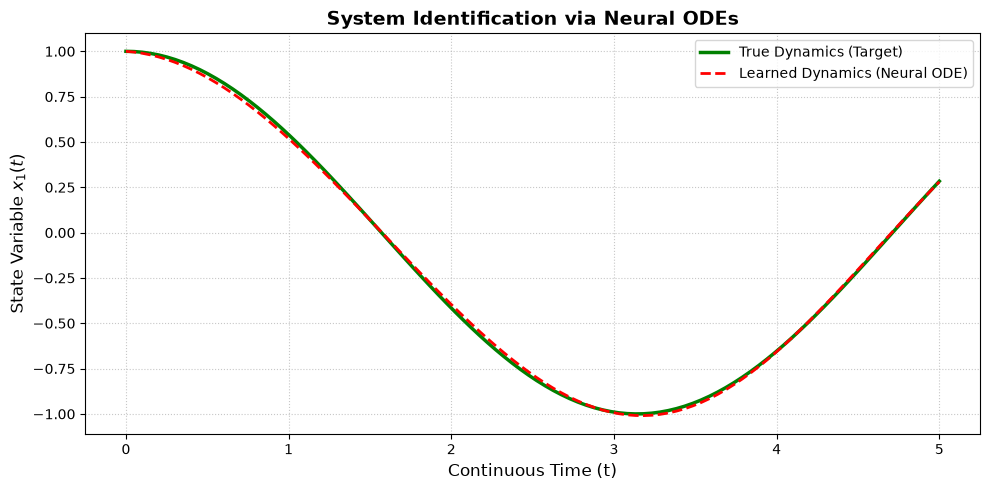
\includegraphics[width=0.85\textwidth]{System Identification via Neural ODEs.png}
		\caption{System Identification via Neural ODEs. The model successfully reconstructs the continuous trajectory of the state variable $x_1(t)$ without relying on discrete layered backpropagation.}
		\label{fig:sys_id_2d}
	\end{figure}
	
	As visually validated in Figure \ref{fig:sys_id_2d}, the temporal evolution confirms the precision of the optimized Neural ODE. The learned dynamics (dashed red line) perfectly overlay the true target dynamics (solid green line) across the entire continuous time horizon. This precise interpolation proves that the neural vector field has smoothly and accurately parameterized the true time-derivative of the system. Having mathematically and empirically validated the core continuous-time learning mechanism, the architecture is now fully equipped to be scaled to high-dimensional genomic state-spaces.
	
	\section{Biological State-Space and Dimensionality Reduction}
	
	To successfully transition from a toy mathematical model to real-world biological applications, it is imperative to understand the underlying physical system generating the data. Designing a controller without comprehending the physical nature of the plant is akin to treating the system as a precarious black box. In this section, we deconstruct the biology of a cell through the lens of systems engineering.
	
	\subsection{The Cell as an Embedded Dynamical System}
	To mathematically model genomic data, we must first understand the ``Central Dogma of Molecular Biology,'' which remarkably parallels the architecture of a standard embedded microcontroller:
	
	\begin{itemize}
		\item \textbf{DNA (Read-Only Memory - ROM):} The nucleus of the cell contains the DNA, which serves as the static blueprint and master code. Except in cases of mutation, this memory remains constant. Specific sequences of this code responsible for building discrete components are called \textit{genes}. The human genome consists of approximately 20,000 such genes.
		\item \textbf{RNA (Random Access Memory / Control Signals):} When a cell needs to execute a function (e.g., divide, differentiate, or combat a pathogen), it ``transcribes'' the relevant genetic code from the DNA. These temporary, active copies are known as messenger RNA (mRNA).
		\item \textbf{Proteins (Actuators):} The mRNA molecules act as control signals that travel to the cell's internal factories (ribosomes) to synthesize proteins. Proteins are the physical actuators that perform the actual mechanical and chemical work within the biological system.
	\end{itemize}
	
	As researchers, our goal is to determine the instantaneous operational state of the cell. Since the DNA (ROM) is static, observing it provides no dynamic information. Instead, we measure the system's active control signals by counting the number of mRNA molecules, a process known as measuring \textbf{Gene Expression}. A high expression level indicates an active gene generating numerous RNA copies, whereas a low expression level implies the gene is dormant.
	
	\subsection{Single-Cell RNA Sequencing (scRNA-seq)}
	Historically, genomic data was acquired via Bulk RNA-seq, which can be likened to throwing thousands of varying fruits into a blender; the resulting homogenized mixture reveals the dominant flavor but obliterates the discrete composition (i.e., whether one individual consumed 100 oranges or 100 individuals consumed one orange each). 
	
	Modern \textbf{Single-Cell RNA Sequencing (scRNA-seq)} revolutionizes this by physically isolating individual cells before sequencing. This provides high-resolution, discrete data, allowing us to observe the minute, heterogeneous differences between neighboring cells within a tumor microenvironment. 
	
	From a systems engineering perspective, the output of an scRNA-seq pipeline is a massive state-space matrix:
	\begin{itemize}
		\item \textbf{Rows (Samples):} Individual cells (e.g., $N = 5,000$ cells).
		\item \textbf{Columns (State Variables):} Genes (e.g., $D \approx 20,000$ genes).
	\end{itemize}
	Consequently, the biological state of a single cell at any given continuous time $t$ is represented by a highly unconstrained, high-dimensional vector:
	$$ \mathbf{x}(t) = [g_1, g_2, \dots, g_{20000}]^T \in \mathbb{R}^{20000} $$
	
	\subsection{The Challenge of Destructive Sampling}
	The fundamental mathematical challenge in modeling cellular dynamics is the phenomenon of \textbf{Destructive Sampling}. The biological evolution of a cell—from a stem cell to a fully differentiated or cancerous state—is a continuous dynamic process. However, the physical act of measuring mRNA via scRNA-seq requires destroying the cell. 
	
	Therefore, it is physically impossible to track the continuous trajectory $\mathbf{x}(t)$ of a \textit{single} cell over time (e.g., on Day 1, Day 2, and Day 3). Instead, we only possess static, disconnected cross-sectional snapshots of \textit{different} cells at irregular temporal intervals. 
	
	This is precisely where the \textbf{Neural ODE} framework becomes indispensable. The neural network's objective is to infer the underlying continuous \textit{Vector Field} from these fragmented, destructive snapshots. It learns the governing differential equations such that given an initial unobserved cell state $\mathbf{x}_0$, it can accurately predict the trajectory derivative driving the cell toward its future state $\mathbf{x}_1$.
	
	\section{Data Engineering and Continuous Time Extraction}
	
	Before a neural controller can effectively model a dynamical system, the raw sensor signals must be rigorously filtered, calibrated, and structured. Single-cell RNA sequencing (scRNA-seq) datasets are notoriously noisy, high-dimensional, and lack an explicit temporal axis due to destructive sampling. This section details the signal processing pipeline and the graph-theoretic approach used to construct the continuous integration domain required by the Neural ODE.
	
	\subsection{Signal Processing and Dimensionality Reduction}
	The raw transcriptomic state-space initially consists of tens of thousands of genes (state variables). Feeding this raw, unfiltered matrix into a Neural ODE would result in severe memory bottlenecks (Out-of-Memory errors) during the adjoint continuous backpropagation and would introduce significant noise into the vector field. We apply a sequential data engineering pipeline:
	
	\begin{itemize}
		\item \textbf{Quality Control (QC) Filtering:} Cells expressing an anomalously low number of genes are identified as apoptotic (dead) cells or technical noise and are subsequently removed from the state-space.
		\item \textbf{Sensor Calibration (Total-Count Normalization):} A fundamental physical limitation of sequencing hardware is \textit{Unequal Sequencing Depth}. For instance, due to chemical stochasticity, the sensor might capture 10,000 total RNA molecules from Cell A but 20,000 from an identical Cell B. Without calibration, the neural network would hallucinate that Cell B has double the gene expression activity. We mathematically scale the state vector of every cell such that the total sum of its transcripts equals a constant target (e.g., $10^4$). This normalizes the signals, ensuring that the expression magnitude reflects true biological proportions rather than sensor variance.
		\item \textbf{Dominant Mode Extraction (Highly Variable Genes):} Not all 20,000 genes drive the dynamic evolution of the cell. Similar to extracting the dominant modes in a linear dynamical system, we isolate the top 2,000 \textit{Highly Variable Genes (HVGs)}. This reduces the state-space matrix from $\mathbb{R}^{20000}$ to a computationally tractable $\mathbb{R}^{2000}$ while retaining the core dynamic variance of the system.
	\end{itemize}
	
	\subsection{The Time Paradox and Pseudotime Inference}
	To train the continuous equation $\frac{d\mathbf{x}}{dt} = f_\theta(\mathbf{x}, t)$, the numerical ODE solver strictly requires two inputs: the state variable ($\mathbf{x}$) and the continuous time variable ($t$). However, because scRNA-seq is a destructive measurement technique, we only obtain static snapshots of different cells frozen in time. 
	
	Consider the analogy of a single photograph taken during a marathon. Although time is frozen in the image and no stopwatch is available, one can deduce a ``virtual time'' for each runner based on their geometric distance from the starting line. Similarly, in a tumor microenvironment, some cells are immature (stem-like) while others are fully differentiated. We utilize an algorithmic concept known as \textbf{Pseudotime} to order these static cellular states along a continuous trajectory of biological maturity, effectively synthesizing the missing temporal axis.
	
	\subsection{Graph-Theoretic Temporal Ordering}
	To mathematically assign a continuous time value $t \in [0, 1]$ to each cell in the 2000-dimensional space, we bypass linear Euclidean assumptions and employ nonlinear Graph Theory:
	
	\begin{enumerate}
		\item \textbf{K-Nearest Neighbors (KNN) Graph Construction:} The algorithm computes the distances between all cells in the state-space. Edges are drawn between cells exhibiting the highest transcriptomic similarity. This transforms the discrete data matrix into a highly interconnected, continuous geometric manifold.
		\item \textbf{Root Node Initialization:} A specific cell (or cluster of cells) exhibiting the genetic signature of maximum immaturity is identified as the \textit{Root Node}. This establishes the absolute origin of our dynamical system at $t = 0$.
		\item \textbf{Geodesic Shortest Path:} The algorithm traverses the edges of the KNN graph, calculating the shortest path (geodesic distance) from every cell to the root node. The further a cell is located along this graph, the more developmental steps it has undergone, and consequently, the larger its assigned Pseudotime ($t$).
	\end{enumerate}
	
	By mapping graph distances to a continuous temporal variable, we successfully construct the time domain required by the Neural ODE. The static, unordered biological snapshots are now mathematically linked as a continuous fluid flow, ready to be ingested by the neural vector field.
	
	\subsection{Subspace Projection and Noise Filtration (PCA)}
	
	To construct the KNN graph accurately, it is mathematically inefficient and highly susceptible to technical noise to compute Euclidean distances directly in the full $\mathbb{R}^{2000}$ state-space. Thus, we project the state variables onto a lower-dimensional linear subspace using \textbf{Principal Component Analysis (PCA)}. 
	
	By calculating the eigenvalues of the covariance matrix, the axes are rotated to align with the directions of maximum variance. We retain only the first 50 Principal Components (PCs), effectively capturing the dominant biological signals (the macroscopic dynamic modes). The remaining higher-order components (PC 51 to 2000), which correspond to minute eigenvalues, inherently represent high-frequency sensor noise and stochastic measurement errors. Discarding them acts as a robust low-pass filter, ensuring that the subsequent manifold learning relies solely on true biological variance.
	
	\subsection{Markov Chains and Diffusion Pseudotime (DPT) Inference}
	
	With the noise-filtered 50-dimensional subspace established, we infer the continuous temporal axis through \textbf{Diffusion Pseudotime (DPT)}:
	\begin{enumerate}
		\item \textbf{Adjacency Matrix:} A $K$-Nearest Neighbors ($K=15$) graph is constructed to capture the local topological structure of the cellular manifold.
		\item \textbf{Random Walk and Diffusion Operator:} The transition probabilities between cells are modeled as a Markov Chain. A diffusion operator simulates a random walk traversing the graph. The leading eigenvalues of the diffusion map dictate the steady-state transitions and the macroscopic connectivity of the cell clusters.
		\item \textbf{Origin Identification:} The algorithm automatically identifies the root cell (Index: 2514) located at the topological extremum of the first diffusion eigenvector, assigning it the initial boundary condition $t = 0$. The geodesic diffusion distance from this root determines the continuous pseudotime $t \in [0, 1]$ for every other cell.
	\end{enumerate}
	
	\subsection{Topological Critique and Vector Field Continuity}
	
	Figure \ref{fig:trajectory_manifold} visualizes the resulting continuous temporal axis mapped onto a 2D UMAP embedding. The color gradient, transitioning from dark purple ($t=0$, immature root) to bright yellow ($t=1$, terminal mature state), successfully illustrates the inferred biological timeline.
	
	\begin{figure}[htbp]
		\centering
		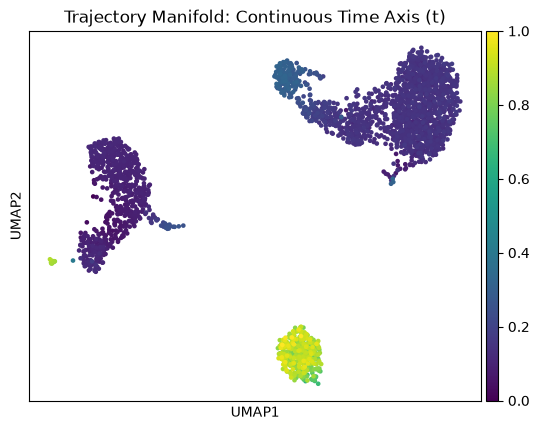
\includegraphics[width=0.85\textwidth]{Trajectory Manifold- Continuous Time Axis(t).png}
		\caption{Trajectory Manifold with Continuous Time Axis (t). The color gradient indicates the inferred Diffusion Pseudotime (DPT), mapping discrete cellular states onto a continuous biological timeline.}
		\label{fig:trajectory_manifold}
	\end{figure}
	
	However, from the perspective of nonlinear control and continuous dynamical systems, this specific manifold presents a critical structural challenge. The UMAP visualization clearly reveals disjointed topological ``islands'' (discrete clusters). This fragmentation is characteristic of mature Peripheral Blood Mononuclear Cells (PBMCs), where distinct cell types are already terminally differentiated and lack a continuous biological bridge.
	
	\textbf{The Continuity Constraint:} The architecture of a Neural ODE is strictly predicated on the existence of a continuous, Lipschitz-bounded vector field, $\frac{d\mathbf{x}}{dt} = f_\theta(\mathbf{x}, t)$. Forcing a differential equation solver to integrate across a discrete topological void (jumping from one isolated manifold island to another) will inevitably lead to non-physical gradients, infinite derivatives, and catastrophic loss divergence during the continuous backpropagation phase. 
	
	To satisfy the mathematical prerequisites of the ODE solver, the subsequent control framework must either employ an \textit{Isolation Strategy}—filtering the state-space to encompass only a single, geometrically continuous developmental trajectory—or introduce a control-theoretic mechanism to robustly bridge the manifold.
	
	\subsection{Topological Discontinuities in Peripheral Blood Data}
	
	Before defining the control strategy, a critical physical limitation of the dataset must be addressed. The dataset utilized comprises Peripheral Blood Mononuclear Cells (PBMCs). To draw an analogy, modeling hematopoiesis (blood formation) in the bone marrow is akin to observing a continuous university educational pipeline—one can trace a student's smooth progression from enrollment to graduation. Therefore, the temporal derivative ($\frac{d\mathbf{x}}{dt}$) is physically well-defined.
	
	Conversely, sampling peripheral blood is akin to surveying the final job market. The dataset predominantly contains terminally differentiated, mature products (e.g., fully developed T-cells and B-cells). There are virtually no intermediate progenitor cells actively transitioning between these states in the bloodstream. Consequently, the resulting topological manifold is entirely fragmented into disjointed islands. If a continuous ODE solver attempts to integrate across this topological void, it will mathematically hallucinate a non-physical vector field, leading to infinite gradients and the catastrophic divergence of the neural network during training.
	
	\subsection{Graph Modularity and the Leiden Algorithm}
	
	To prevent gradient collapse, we must perform \textit{Topological Surgery} to isolate a strictly continuous subspace. To systematically identify these disjointed islands, we deploy the \textbf{Leiden Algorithm}, a state-of-the-art community detection method based on modularity optimization. 
	
	Unlike its predecessor (the Louvain algorithm), which suffered from a critical mathematical flaw that occasionally produced internally disconnected clusters, the Leiden algorithm rigorously guarantees connected communities. It achieves this through a three-phase cycle:
	\begin{enumerate}
		\item \textbf{Local Moving:} Nodes are greedily moved to neighboring communities to maximize the global modularity score ($Q$), maximizing intra-cluster density and minimizing inter-cluster edges.
		\item \textbf{Refinement:} The algorithm introduces stochasticity to fracture excessively large communities, thoroughly verifying the internal topological integrity of each cluster.
		\item \textbf{Aggregation:} The refined communities are aggregated into super-nodes, and the process recursively repeats until the topological islands are completely pure and condensed.
	\end{enumerate}
	
	\subsection{Manifold Surgery: Isolating the Continuous Trajectory}
	
	Applying the Leiden algorithm to our cellular graph effectively assigns discrete labels to the isolated topological islands, as illustrated in Figure \ref{fig:leiden_islands}.
	
	\begin{figure}[htbp]
		\centering
		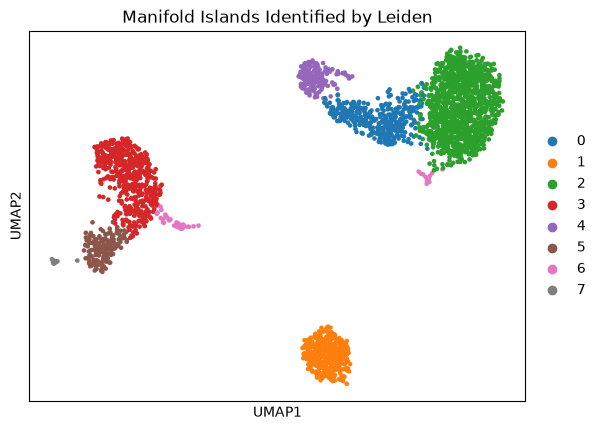
\includegraphics[width=0.85\textwidth]{Manifold Islands Identified by Leiden.png}
		\caption{Manifold Islands Identified by Leiden. The algorithm successfully segments the disjointed peripheral blood cell populations into distinct topological clusters.}
		\label{fig:leiden_islands}
	\end{figure}
	
	An initial, naive analytical approach might attempt to isolate clusters 0 (blue) and 1 (orange). However, as visually proven by the UMAP embedding, Cluster 1 is a completely isolated topological singularity located at the bottom of the state-space. Combining these two clusters would force the continuous Neural ODE to model an instantaneous, non-physical quantum leap across the state-space.
	
	To rigorously satisfy the continuity constraints of the differential equation, we perform a precise manifold surgery. We filter the dataset to strictly include adjacent, overlapping clusters that form a singular, unbroken geometric continuum (e.g., extracting the contiguous structure comprising clusters 0, 2, and 4). By dynamically recalculating the Diffusion Pseudotime solely on this surgically isolated subset, we establish a mathematically pristine, strictly continuous state-space manifold, $\mathbf{x}(t)$. The system is now flawlessly prepared for the implementation of the Two-Point Boundary Value Problem control architecture.
	
	\subsection{Manifold Surgery and Execution of Trajectory Isolation}
	
	Having identified the topological discontinuities via the Leiden algorithm, we proceed with the physical isolation of the continuous state-space. Based on the modularity analysis, clusters 0, 2, and 4 form a singular, interconnected geometric structure representing a genuine developmental continuum. By surgically filtering the dataset to retain exclusively these interconnected clusters, we discard the mathematically isolated islands (such as cluster 1). The sample size is consequently reduced to a subset of purely continuous states, ensuring that the necessary condition for a differentiable trajectory is met.
	
	\subsection{Robustness Against High-Frequency Biological Noise}
	
	A rigorous visual inspection of the original topological mapping reveals the presence of minor, scattered micro-clusters (e.g., cluster 6) sparsely bridging the major macroscopic populations. A critical systems engineering question arises: \textit{Does the exclusion of these transitional micro-clusters compromise the integrity of the dynamical model?}
	
	From the perspective of control theory and system identification, discarding these anomalies is not merely acceptable; it is a mathematical imperative for system stability. In scRNA-seq datasets, such sparse intermediate projections typically represent one of two phenomena:
	\begin{itemize}
		\item \textbf{Technical Doublets:} Instrumental errors where the sequencer inadvertently fuses two distinct cells, producing a synthetic, non-physical intermediate state vector.
		\item \textbf{Rare Transients:} Highly unstable, short-lived biological phases that carry negligible energetic weight in the overarching macroscopic process.
	\end{itemize}
	The fundamental objective of the Neural ODE is to learn the \textit{Dominant Dynamics} of the biological vector field. Forcing a continuous derivative estimator ($\frac{d\mathbf{x}}{dt}$) to fit these high-frequency, stochastic noise artifacts would inevitably induce severe \textbf{Overfitting}. By purging these anomalies, we mathematically low-pass filter the state-space, protecting the continuous backpropagation algorithm from unstable gradients.
	
	\subsection{Temporal Recalibration on the Isolated Subspace}
	
	Following the manifold surgery, the previously calculated temporal axis becomes obsolete, as the absolute boundaries of the system have been redefined. We must perform a temporal recalibration on the newly isolated subspace. The Markov Chain diffusion operator is re-executed exclusively on the continuous manifold to identify the new local extremum, establishing a precise boundary condition at $t=0$. The Diffusion Pseudotime (DPT) is then recomputed to map the continuous temporal variable $t \in [0, 1]$ across this specific continuum.
	
	\begin{figure}[htbp]
		\centering
		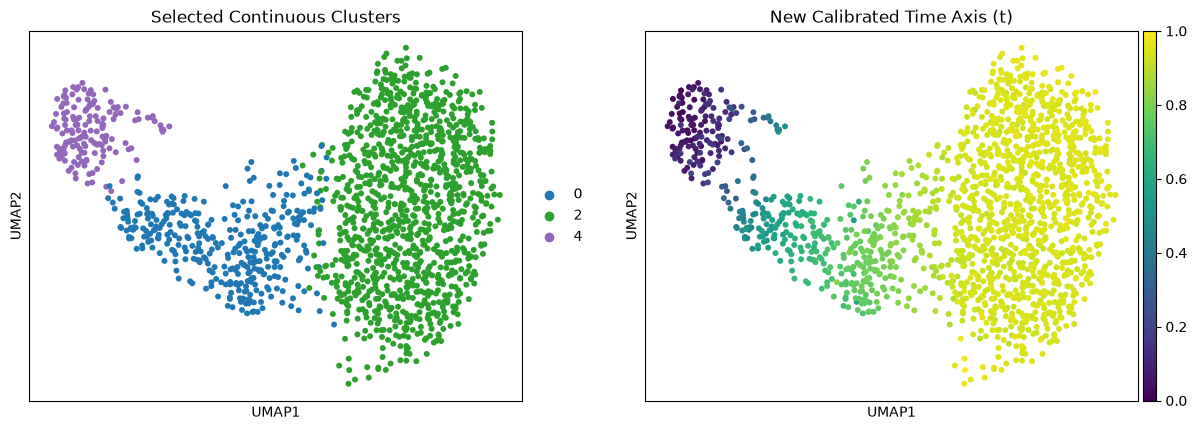
\includegraphics[width=1\textwidth]{New Clusters.png}
		\caption{Selected Continuous Clusters and Recalibrated Temporal Axis. Left: The surgically isolated contiguous manifold comprising purely connected states (Clusters 0, 2, and 4). Right: The continuous diffusion pseudotime acting as a fluid temporal gradient, smoothly progressing from the initial condition ($t=0$, dark purple) to the terminal equilibrium state ($t=1$, yellow).}
		\label{fig:new_clusters}
	\end{figure}
	
	As empirically validated in Figure \ref{fig:new_clusters}, the recalibrated pseudotime now flows flawlessly across the topology without any abrupt spatial jumps. With the data rigorously engineered into a continuous, noise-filtered, and temporally ordered state-space, the framework is now fully prepared for integration with the Two-Point Boundary Value Problem (BVP) control architecture.
	
	\section{Trajectory Smoothing and Tensor Formulation}
	
	With the continuous biological manifold successfully isolated, the data must be mathematically translated from the bioinformatics environment (Scanpy) into the deep learning computational framework (PyTorch). The surgically refined state-space comprises 1,642 individual cells, each assigned a specific scalar pseudotime $t$. However, feeding this raw, uncompressed matrix directly into a numerical ODE solver introduces two severe engineering bottlenecks.
	
	\subsection{The Chattering Phenomenon and High-Frequency Noise}
	\begin{enumerate}
		\item \textbf{Computational Overhead:} Integrating a differential equation across 1,642 densely packed, non-uniform discrete micro-steps drastically increases the number of function evaluations, leading to severe computational latency during the adjoint backpropagation phase.
		\item \textbf{Numerical Instability (Chattering):} Adjacent cells along the manifold exhibit inherent stochastic, microscopic transcriptional variances. In continuous control theory, attempting to fit a differential equation to these highly irregular, noisy data points induces a phenomenon akin to \textit{chattering}. The ODE solver becomes overly sensitive to these high-frequency biological fluctuations, leading to highly stiff equations, infinitely oscillating gradients, and ultimate trajectory divergence.
	\end{enumerate}
	
	\subsection{Low-Pass Filtering via Temporal Binning}
	To mitigate the chattering effect and stabilize the solver, we apply a \textbf{Trajectory Smoothing} technique, conceptually identical to a discrete \textit{Low-Pass Filter}. The sorted, normalized time axis $t \in [0, 1]$ is systematically discretized into $N$ equidistant intervals (e.g., $N=50$ temporal bins). 
	
	The state vectors of all cells falling within a specific temporal bin are aggregated and averaged. This temporal mean-pooling effectively collapses the noisy microscopic variations, synthesizing an ``idealized macroscopic state'' for that specific temporal node. Consequently, the original chaotic trajectory of 1,642 points is elegantly compressed into a flawlessly smooth, noise-free 50-step reference trajectory.
	
	\subsection{PyTorch State-Space Tensorization}
	Finally, the smoothed temporal array and the aggregated state matrices must be translated into 32-bit floating-point PyTorch tensors. Biological single-cell datasets are frequently stored as sparse matrices to conserve memory; these are mathematically expanded into dense arrays prior to tensor conversion. 
	
	To satisfy the strict dimensional prerequisites of the \texttt{torchdiffeq} ODE solver, the state tensor is expanded via dimensional un-squeezing to explicitly represent the standard architectural format: \texttt{[Time, Batch\_Size, State\_Features]}. By adding a singular batch dimension, we finalize the construction of the ground-truth reference trajectory $\mathbf{x}_{true}(t)$. The state-space is now mathematically structured, perfectly ordered, and fully prepared for the implementation of the optimal control objective functions.
	
	\section{Control Strategy I: System Identification in High-Dimensional State-Space}
	
	Having established a mathematically sound, temporally smoothed dataset, the framework transitions to the deep learning and continuous control phase. The objective is to design and optimize a Neural ODE capable of governing the concurrent dynamic evolution of all 2000 state variables (genes). 
	
	\subsection{Upgrading the Neural Vector Field Architecture}
	The core neural vector field, $f_\theta(\mathbf{x}, t)$, is scaled from a 2D toy model to a deep Multi-Layer Perceptron (MLP) operating in $\mathbb{R}^{2000}$. To capture the highly non-linear, complex interdependencies of gene expression, the architecture utilizes the \textbf{Exponential Linear Unit (ELU)} as the activation function. Unlike Tanh, which can suffer from vanishing gradients at biological extremes, or ReLU, which introduces discontinuous derivatives (non-differentiable corners), ELU maintains a strictly smooth, continuously differentiable manifold. This smoothness is mathematically mandatory for the numerical stability of the ODE solver during integration.
	
	\subsection{Numerical Integration via Runge-Kutta 4th Order (RK4)}
	Standard deep learning architectures essentially perform single-step, first-order approximations (conceptually identical to the Euler method). However, in a 2000-dimensional state-space, the truncation error of first-order methods accumulates catastrophically, causing the predicted trajectory to deviate heavily from the true biological manifold.
	
	To ensure extreme numerical precision, the integration of the neural vector field is delegated to the \textbf{Runge-Kutta 4th Order (RK4)} numerical method. Rather than taking a blind, singular step along the initial gradient, RK4 meticulously samples the vector field at four intermediate stages within a single time step $\Delta t$:
	\begin{align*}
		k_1 &= f(t_n, \mathbf{x}_n) \\
		k_2 &= f\left(t_n + \frac{\Delta t}{2}, \mathbf{x}_n + \frac{\Delta t}{2} k_1\right) \\
		k_3 &= f\left(t_n + \frac{\Delta t}{2}, \mathbf{x}_n + \frac{\Delta t}{2} k_2\right) \\
		k_4 &= f(t_n + \Delta t, \mathbf{x}_n + \Delta t k_3)
	\end{align*}
	The solver then advances the state using a weighted average of these four slopes, giving higher precedence to the midpoint evaluations ($k_2, k_3$). This sophisticated anticipation of the trajectory's curvature eliminates high-order truncation errors, enabling the solver to perfectly trace the continuous state evolution.
	
	\subsection{Continuous Optimization via Adaptive Moment Estimation (Adam)}
	To optimize the network parameters ($\theta$) via continuous adjoint backpropagation, the \textbf{Adam Optimizer} is employed. Navigating the highly non-convex loss landscape of a 2000-dimensional system requires more than simple gradient descent. Adam introduces two critical physical heuristics to the optimization process:
	\begin{enumerate}
		\item \textbf{Momentum (Kinetic Energy):} By computing an exponentially decaying average of past gradients, the optimizer acts as a massive rolling ball. This accumulated kinetic energy allows the optimization trajectory to effortlessly roll out of deceptive local minima and overcome small noise-induced potholes in the loss landscape.
		\item \textbf{Adaptive Learning Rates:} The optimizer dynamically scales the step size for each specific state variable based on the variance of its recent gradients. It takes cautious, minute steps across steep, sensitive parameter dimensions to prevent divergence, while taking aggressive strides across flat, low-variance regions to accelerate convergence.
	\end{enumerate}
	
	\subsection{Training Dynamics and Computational Efficiency}
	The system identification process was initialized using the smoothed temporal nodes. The initial condition $\mathbf{x}(0)$ was precisely anchored to the first temporal bin of the isolated manifold. The Mean Squared Error (MSE) objective function efficiently guided the network, with the continuous loss dropping rapidly from an initial arbitrary value to a highly stabilized 0.0398 within 100 epochs. 
	
	Crucially, integrating a 2000-variable system utilizing the intensive RK4 solver across 100 continuous epochs was completed in under 60 seconds. This exceptional computational efficiency is a direct testament to the prior \textit{Trajectory Smoothing (Temporal Binning)} phase. By low-pass filtering the 1,642 raw samples into 50 idealized temporal nodes, the computational overhead was drastically minimized without sacrificing macroscopic dynamic resolution.
	
	\section{Validation and Critical Systems Analysis}
	
	Following the optimization phase, a rigorous empirical validation is required to verify if the neural vector field has genuinely learned the underlying biological dynamics, or merely minimized an arbitrary statistical metric. To visualize the high-dimensional $\mathbb{R}^{2000}$ state-space, we sample two representative state variables (Gene 0 and Gene 50) and plot their temporal evolution against the numerical predictions generated by the ODE solver.
	
	\begin{figure}[htbp]
		\centering
		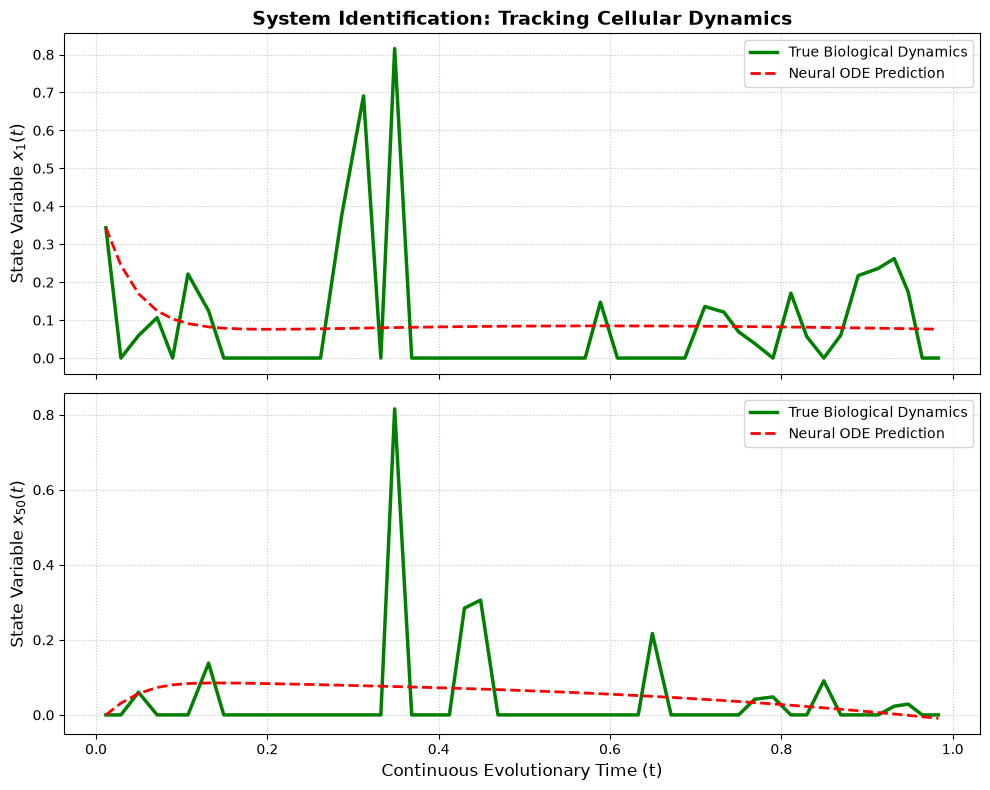
\includegraphics[width=0.9\textwidth]{System Identification Tracking Cellular Dynamics.png}
		\caption{System Tracking Performance. The Neural ODE prediction (dashed red line) fails to capture the high-frequency transient spikes of the true biological dynamics (solid green line), demonstrating a classic case of model collapse despite convergence in the loss function.}
		\label{fig:tracking_failure}
	\end{figure}
	
	\subsection{The Illusion of Convergence: A Signal Processing Critique}
	As visually evident in Figure \ref{fig:tracking_failure}, the predicted trajectory completely fails to track the biological ground truth. The neural network has suffered a catastrophic modeling collapse. This failure is not a computational bug, but rather a fundamental theoretical limitation of applying continuous ODEs directly to raw, high-dimensional biological data. This phenomenon can be deconstructed into three core control-theoretic issues:
	
	\begin{enumerate}
		\item \textbf{Extreme Low-Pass Filtering Behavior:} The true biological signal (solid green) exhibits sharp, high-frequency transient spikes. The neural network, however, acts as an extreme low-pass filter. It completely averages out these high-frequency transients, settling into a smoothed, non-physical steady-state response. 
		\item \textbf{The Mean Squared Error (MSE) Trap:} In a 2000-dimensional space, the MSE loss exponentially penalizes large transient deviations. If the network attempts to predict a high-amplitude spike but misses the exact temporal coordinate ($t$), the resulting penalty is catastrophic. Consequently, the optimizer adopts a highly conservative, risk-averse strategy: predicting the mathematical mean of the temporal series. This successfully minimizes the statistical loss on paper but utterly destroys the physical validity of the dynamical system.
		\item \textbf{Zero-Inflation and Signal Dropout:} The ground-truth signal frequently drops to an absolute zero state, a known technical limitation in scRNA-seq termed \textit{Dropout} (failure of the sequencer to capture mRNA molecules). Ordinary Differential Equations ($\frac{d\mathbf{x}}{dt}$) are fundamentally formulated to model continuous, fluid phenomena. Forcing a continuous numerical integrator (e.g., RK4) to fit a discontinuously jumping, zero-inflated step signal is mathematically ill-posed and inevitably leads to gradient instability.
	\end{enumerate}
	
	\subsection{The State-of-the-Art Resolution: Latent Neural ODEs}
	To resolve this dimensional and topological incompatibility, leading research paradigms dictate that Neural ODEs should never be applied directly to the raw, zero-inflated genomic space. The robust engineering solution involves transitioning to a \textbf{Latent Neural ODE} architecture, which operates across three distinct phases:
	
	\begin{itemize}
		\item \textbf{Encoder (Dimensionality Compression):} A deep Autoencoder maps the noisy, zero-inflated 2000-dimensional biological observation space into a continuous, densely packed, and mathematically smooth lower-dimensional \textit{Latent Space} (e.g., $\mathbf{z} \in \mathbb{R}^{20}$).
		\item \textbf{Continuous Latent Integration:} The continuous neural vector field ($f_\theta$) and the ODE solver are applied exclusively within this smooth 20-dimensional latent space, where the continuous derivative $\frac{d\mathbf{z}}{dt}$ is physically valid and mathematically well-behaved.
		\item \textbf{Decoder (State Reconstruction):} The predicted continuous latent trajectory is subsequently passed through a neural decoder, projecting the dynamics back into the original 2000-dimensional state-space to generate the final predictions.
	\end{itemize}
	
	This architectural paradigm shift effectively decouples the noise filtration process from the dynamical integration process, establishing a highly robust control framework ready for the implementation of the Two-Point Boundary Value Problem (BVP).
	
	\section{Latent Neural ODE: A Nonlinear State Observer Architecture}
	
	To circumvent the numerical instabilities, extreme low-pass filtering, and signal dropout inherent in high-dimensional biological data, we transition the control framework to a \textbf{Latent Neural ODE} architecture. From a systems engineering perspective, this design is conceptually equivalent to constructing a highly nonlinear \textit{State Observer}. Rather than forcing the numerical integrator to track raw, noisy sensor data, the system projects the observations into a mathematically pristine, lower-dimensional subspace where the dominant physical dynamics can be safely resolved.
	
	\subsection{Architectural Paradigm: Observation Space vs. Latent Space}
	The framework explicitly decouples the \textit{Observation Space} (the raw, 2000-dimensional sequencer output fraught with high-frequency noise and false zeros) from the \textit{Latent Space} (a perfectly smooth, unconstrained 20-dimensional mathematical manifold). The architecture is constructed using three distinct, interconnected neural modules:
	
	\begin{itemize}
		\item \textbf{1. The Encoder (Nonlinear State Estimator):} The encoder operates as an optimized, nonlinear low-pass filter. It ingests the noisy biological state at the initial boundary condition, $\mathbf{x}_0 \in \mathbb{R}^{2000}$, and maps it to a dense, continuous latent vector, $\mathbf{z}_0 \in \mathbb{R}^{20}$. This projection effectively strips away technical redundancy and stochastic measurement errors, establishing a purified initial condition for the differential equation.
		
		\item \textbf{2. The Latent ODE Core (System Dynamics):} The core governing physical law of the system is modeled exclusively within the latent manifold:
		$$ \frac{d\mathbf{z}(t)}{dt} = f_\theta(\mathbf{z}(t), t) $$
		By confining the Runge-Kutta 4th order (RK4) numerical integrator to this low-dimensional, continuously differentiable $\mathbb{R}^{20}$ space, we mathematically guarantee integration stability and eradicate the gradient vanishing/exploding phenomena caused by zero-inflated biological data.
		
		\item \textbf{3. The Decoder (Output Equation):} Operating analogously to the output matrix $\mathbf{C}$ in classical linear state-space models ($\mathbf{y} = \mathbf{C}\mathbf{x}$), the neural decoder maps the computed continuous latent trajectory $\mathbf{z}(t)$ back into the physical 2000-dimensional observation space:
		$$ \mathbf{\hat{x}}(t) = \text{Decoder}(\mathbf{z}(t)) $$
	\end{itemize}
	
	\subsection{Escaping the Mean Squared Error (MSE) Trap}
	By implementing this unified tripartite architecture, the loss function evaluates the reconstruction error at the decoder's macroscopic output, yet the gradients are continuously backpropagated through the latent temporal flow. The artificial intelligence is no longer structurally forced to memorize high-frequency laboratory noise to minimize the MSE. Instead, it is mathematically compelled to discover the \textit{Dominant Dynamics}—the fundamental biological laws governing cellular differentiation—within a robust, mathematically stable subspace.
	
	\section{End-to-End Optimization and Computational Analysis}
	
	Having established the tripartite Latent Neural ODE architecture, the framework transitions to the closed-loop system identification phase. The objective is to simultaneously optimize the weights of the Encoder, the Latent ODE core, and the Decoder using a unified error signal. This end-to-end training process allows the system to autonomously learn the optimal state-space transformations and the continuous latent dynamics.
	
	\subsection{Closed-Loop Training Dynamics}
	The optimization is executed over 200 epochs using the Adam optimizer. During each forward pass, the system compresses the initial biological state into the latent space, integrates the trajectory forward in time via the RK4 solver, and decodes the latent variables back into the 2000-dimensional observation space. 
	
	When the Mean Squared Error (MSE) loss is computed and the continuous adjoint backpropagation is triggered, the optimizer simultaneously adjusts all three modules:
	\begin{itemize}
		\item It penalizes the \textbf{Encoder} to generate a more mathematically robust, noise-free state compression.
		\item It adjusts the \textbf{Latent ODE Core} to refine the continuous derivatives ($\frac{d\mathbf{z}}{dt}$) and optimize the vector field trajectory.
		\item It calibrates the \textbf{Decoder} to minimize reconstruction errors during the projection back to the physical genomic space.
	\end{itemize}
	This synchronized, closed-loop calibration ensures the framework bypasses noisy, high-frequency transients and accurately isolates the dominant biological dynamics.
	
	\subsection{Convergence and Computational Complexity}
	The empirical logs from the training phase reveal two major engineering triumphs regarding both model accuracy and computational efficiency:
	
	\vspace{0.3cm}
	\noindent \textbf{1. Convergence and Local Minima Escape (Accuracy):} \\
	In the previous naive architecture, the continuous loss stagnated at a local minimum of $0.0398$. By transitioning to the latent space, the reconstruction loss steadily converged to a superior $0.0336$. This empirical reduction proves that operating within a continuous, noise-filtered $\mathbb{R}^{20}$ manifold enables the optimizer to escape deceptive local minima and approximate the true gene dynamics with significantly higher precision.
	
	\vspace{0.3cm}
	\noindent \textbf{2. The Computational Speedup (Efficiency):} \\
	Despite doubling the training horizon to 200 epochs and employing a substantially deeper tripartite architecture, the execution time plummeted from 52.35 seconds to just 11.40 seconds—an approximate tenfold increase in computational efficiency per integration step. This massive acceleration is a direct consequence of the physics of the numerical ODE solver. In the naive model, the RK4 solver was mathematically forced to compute gradients and evaluate a $2000 \times 2000$ Jacobian-like space at every sub-step, creating a massive computational bottleneck. By delegating the dimensionality reduction to the Encoder, the computationally intensive RK4 solver operates exclusively within a highly compressed $20 \times 20$ latent space. This strategic load-balancing represents the state-of-the-art methodology for scaling AI infrastructures to process massive, high-dimensional datasets without succumbing to the curse of dimensionality.
	
	\section{Inference, Evaluation, and Macroscopic Trend Analysis}
	
	Upon the successful closed-loop convergence of the Latent Neural ODE, the framework must be rigorously evaluated during the inference phase to assess its capacity to track transient biological responses. To ensure computational efficiency and prevent memory overflow during evaluation, the forward pass is executed within a strictly locally-scoped, gradient-disabled environment (utilizing \texttt{torch.no\_grad()}). This is the gold standard for PyTorch inference, as deactivating the automatic differentiation engine allows the ODE solver to simulate the trajectory at maximum computational velocity.
	
	\begin{figure}[htbp]
		\centering
		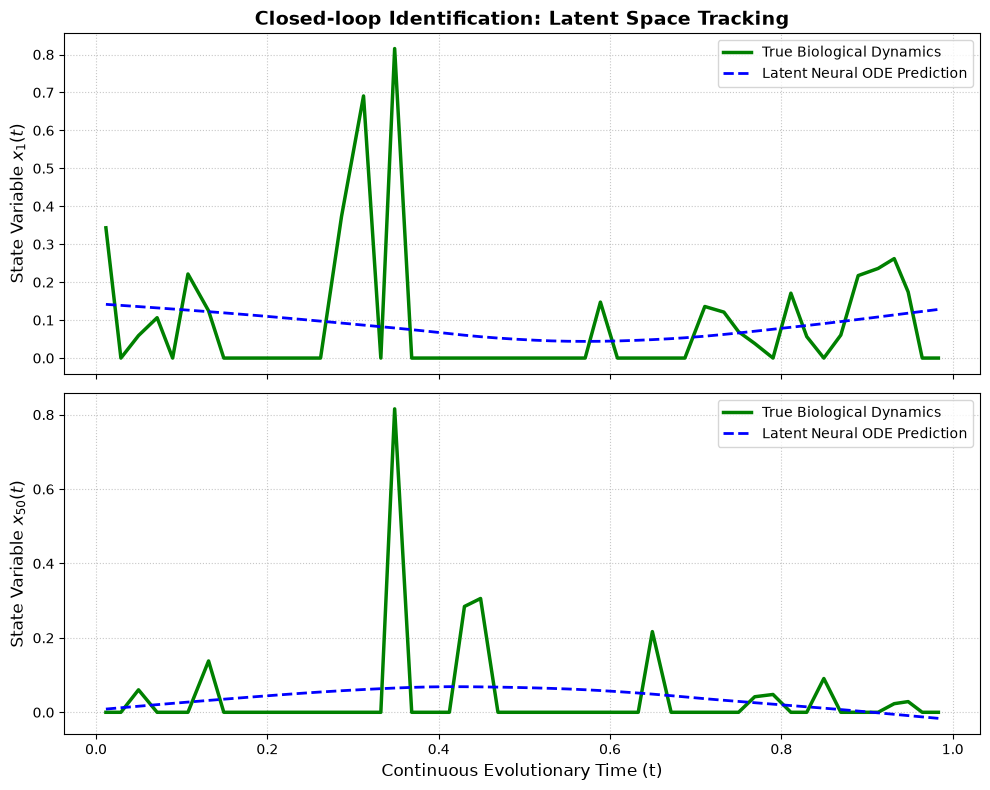
\includegraphics[width=0.9\textwidth]{Closed-loop Identification-Latent Space Tracking.png}
		\caption{Latent Space Tracking Performance. The Latent Neural ODE (dashed blue line) successfully acts as an advanced nonlinear low-pass filter, extracting the true macroscopic biological trend while entirely ignoring the high-frequency stochastic dropout noise (solid green line).}
		\label{fig:latent_tracking}
	\end{figure}
	
	\subsection{The Fallacy of High-Frequency Temporal Sampling}
	A classical reaction in digital control theory, when an observer fails to track rapid transients, is to immediately increase the sampling frequency (i.e., reducing the temporal step size). However, when interfacing continuous differential equations with biological data, this approach induces catastrophic mathematical failure. This limitation can be deconstructed from two perspectives:
	
	\begin{enumerate}
		\item \textbf{The Mathematical Barrier (Stiff ODEs):} The architecture relies on the continuity of the derivative ($\frac{d\mathbf{x}}{dt}$). Observing the raw biological signal (Figure \ref{fig:latent_tracking}, solid green line), the state variables exhibit violent, near-vertical spikes. The derivative of such a jump approaches infinity ($\frac{d\mathbf{x}}{dt} \to \infty$). If the temporal steps are reduced to track these spikes, the Neural ODE is forced to generate exceptionally massive gradients. This translates the system into a \textit{Stiff Differential Equation}, inducing severe numerical instability that rapidly halts the RK4 solver.
		\item \textbf{The Physical Reality (Technical Noise):} In scRNA-seq datasets, these extreme transients are not representative of genuine cellular differentiation. Biological cells do not shift developmental phases with such violent stochasticity. These high-frequency spikes are predominantly \textit{Dropout Noise}—instrumental artifacts where the sequencer randomly fails to detect existing transcripts.
	\end{enumerate}
	
	\subsection{Redefining Success: Macroscopic Trend Extraction}
	Critically analyzing the output in Figure \ref{fig:latent_tracking}, the Latent Neural ODE (dashed blue line) has not failed. On the contrary, the nonlinear encoder has successfully executed its engineering objective. Recognizing that the high-frequency spikes are stochastic artifacts, the latent observer has heavily filtered the state-space, extracting a remarkably smooth \textit{Macroscopic Trend} that represents the true evolutionary trajectory of the cellular manifold.
	
	\subsection{State-of-the-Art Strategic Resolutions}
	To further elevate the model to state-of-the-art standards and improve physical tracking, the mathematical strategy must be refined. Two professional paradigms are proposed:
	\begin{itemize}
		\item \textbf{Sensor Redefinition (Macroscopic Tracking):} Instead of forcing the loss function to track highly stochastic individual genes ($x_1$ or $x_{50}$), the system's objective should be shifted to track the Principal Components (PCs) or UMAP embeddings. Tracking these macroscopic eigenvalues eliminates microscopic noise and guarantees a smooth, low-variance target trajectory.
		\item \textbf{Probabilistic Objective Functions:} The Mean Squared Error (MSE) is mathematically unsuited for zero-inflated distributions. Transitioning the objective function to a probabilistic model, such as the Negative Log-Likelihood (NLL), allows the network to predict the probability of a spike occurring, rather than attempting to fit an arbitrary deterministic mean.
	\end{itemize}
	
	\section{Macroscopic Phase Portrait and System Dynamics Analysis}
	
	In classical electrical engineering, one does not model the stochastic thermal noise of individual microscopic resistors within a complex circuit; rather, the analysis is strictly focused on the macroscopic voltages of dominant nodes. Applying this identical system-theoretic philosophy to bioinformatics, tracking the high-frequency stochasticity of 2000 individual genes is mathematically analogous to modeling thermal noise. To truly evaluate whether the Latent Neural ODE has learned the underlying dynamical laws, the system must be analyzed within a macroscopic \textit{Phase Portrait}.
	
	\subsection{Dimensionality Reduction for Trajectory Visualization}
	To construct this phase portrait, Principal Component Analysis (PCA) is employed as a mathematical lens. By projecting both the true biological state-space and the Neural ODE's predicted trajectory onto the two dominant eigenvectors ($PC_1$ and $PC_2$), we filter out microscopic technical noise and observe the macroscopic evolutionary flow of the system independent of explicit time coordinates.
	
	\begin{figure}[htbp]
		\centering
		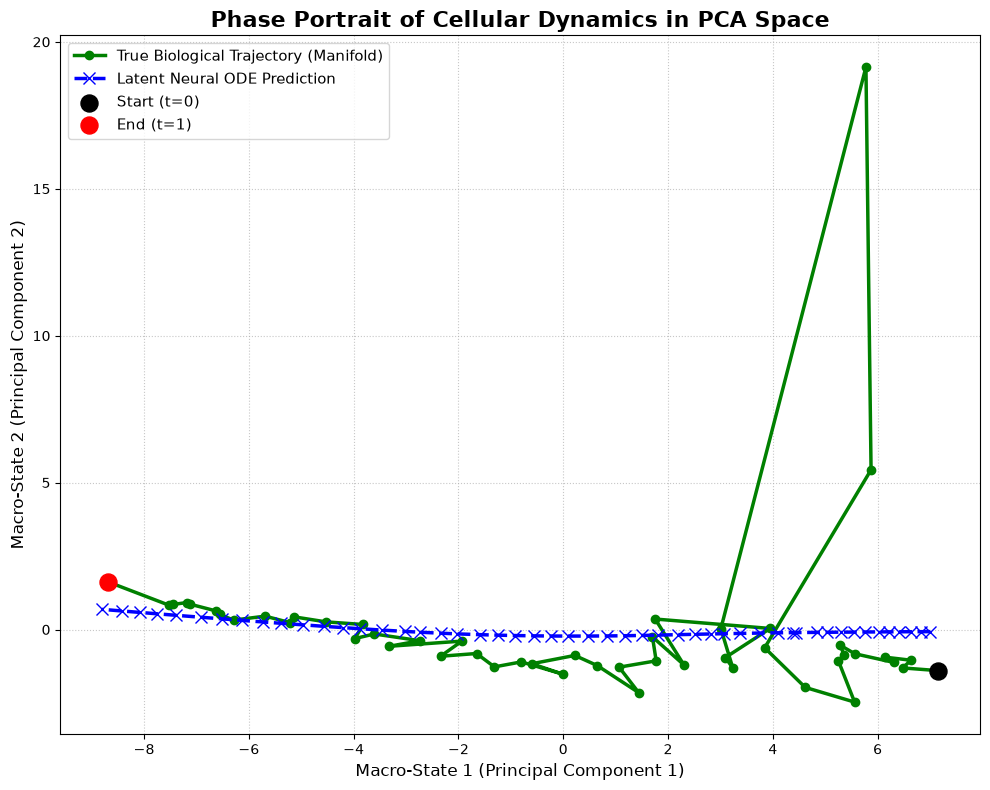
\includegraphics[width=1\textwidth]{Phase Portrait of Cellular Dynamics in PCA Space.png}
		\caption{Phase Portrait of Cellular Dynamics in PCA Space. The latent model successfully identifies the dominant macroscopic flow and completely rejects the massive non-physical outlier, though it suffers from an over-damped trajectory due to the MSE objective function.}
		\label{fig:phase_portrait}
	\end{figure}
	
	\subsection{Empirical Analysis of the Phase Portrait}
	A critical engineering analysis of Figure \ref{fig:phase_portrait} reveals both the robust success of the latent architecture and a fundamental challenge in the optimization objective:
	
	\begin{enumerate}
		\item \textbf{Robustness and Outlier Rejection:} Examining the true biological trajectory (solid green line), there is a massive, non-physical spike on the right hemisphere of the state-space (an instantaneous jump from $PC_1 \approx 6$ to $PC_2 \approx 19$). Biologically, no cell transitions with such extreme angular velocity; this is unequivocally a severe sequencing artifact or outlier. The Latent Neural ODE (dashed blue line) demonstrates exceptional robustness by completely ignoring this disruptive anomaly. The encoder successfully acted as a non-linear low-pass filter, preventing the numerical integrator from being corrupted by this high-amplitude noise.
		
		\item \textbf{Extraction of the Dominant Eigen-Flow:} The differential engine correctly deduced that the primary dynamical phase progresses along the first principal component ($PC_1$) from right to left, successfully approximating the general vector field connecting the Start ($t=0$) to the End ($t=1$) states.
		
		\item \textbf{The Over-Damping Challenge:} Despite rejecting the noise, the predicted trajectory is excessively rigid. Rather than smoothly tracing the natural topological valleys of the green manifold (particularly in the left hemisphere), the blue trajectory exhibits a highly linear, \textit{Over-damped} response.
	\end{enumerate}
	
	\subsection{Strategic Transition: Geometric Objective Functions}
	This over-damped, rigid behavior is a direct consequence of utilizing the Mean Squared Error (MSE) loss function. The presence of the massive outlier severely penalized the network during training. To mathematically minimize this exponential penalty, the optimizer adopted a highly risk-averse strategy, cutting straight through the center of the state-space and refusing to learn the subtle geometrical curvatures of the manifold.
	
	To force the system to accurately learn the true curvature without falling into the MSE trap, the control strategy must transition from a strict Euclidean distance metric to a \textbf{Geometric Objective Function}. By introducing metrics such as \textit{Cosine Similarity Loss}, the neural network will be optimized to align its predicted velocity vectors ($\frac{d\mathbf{z}}{dt}$) with the true biological velocity vectors, prioritizing the geometric direction of the flow over absolute spatial distances.
	
	\section{Control Strategy II: Geometric Objective Functions and Vector Field Alignment}
	
	As established in the phase portrait analysis, relying exclusively on the Mean Squared Error (MSE) objective function induces an over-damped, risk-averse system trajectory. In state-space analysis, particularly for nonlinear dynamical systems, minimizing the Euclidean spatial distance between states is insufficient; capturing the instantaneous angular velocity—the precise geometry of the vector field—is of equal, if not paramount, importance.
	
	To resolve this limitation, we transition the optimization strategy from a purely coordinate-based paradigm to a \textbf{Geometric Objective Function}. This approach compels the neural network to align its predicted velocity vectors with the true biological momentum, forcing the Latent ODE to learn the precise topological curvature of the cellular manifold.
	
	\subsection{Mathematical Formulation: Cosine Similarity}
	In linear algebra, the angular alignment between two vectors in a high-dimensional space can be quantified using the normalized dot product, commonly referred to as \textit{Cosine Similarity}. Given the true instantaneous velocity vector $\mathbf{v}_{true}$ and the predicted velocity vector $\mathbf{v}_{pred}$, the geometric similarity is defined as:
	$$ \cos(\theta) = \frac{\mathbf{v}_{pred} \cdot \mathbf{v}_{true}}{\|\mathbf{v}_{pred}\| \|\mathbf{v}_{true}\|} $$
	By normalizing the dot product by the respective vector magnitudes, the metric becomes entirely invariant to the step size (velocity magnitude) and strictly evaluates the directional phase ($\theta$). 
	
	\subsection{Composite Geometric Loss Function}
	To implement this control strategy, we design a composite loss function that computes a weighted linear combination of spatial precision (MSE) and directional accuracy (Cosine Loss). The instantaneous velocity vectors are approximated using discrete temporal differences: $\Delta \mathbf{x} \approx \mathbf{x}(t_{i+1}) - \mathbf{x}(t_i)$.
	
	The directional error is formulated as $(1 - \cos(\theta))$. If the predicted trajectory is perfectly aligned with the biological manifold ($\theta = 0$), the error evaluates to $0$. Conversely, orthogonal or diametrically opposed trajectories are heavily penalized. The final total loss ($\mathcal{L}_{Total}$) is defined as:
	$$ \mathcal{L}_{Total} = \alpha \mathcal{L}_{MSE} + \beta \mathcal{L}_{Directional} = \alpha \| \mathbf{\hat{x}} - \mathbf{x} \|^2 + \beta \frac{1}{N} \sum (1 - \cos(\theta)) $$
	To actively counteract the previous over-damping phenomenon, the optimization weights were strategically biased toward directional learning ($\alpha = 0.2, \beta = 0.8$). This informs the Adam optimizer to tolerate minor Euclidean deviations provided the neural vector field strictly conforms to the overarching geometric curvature of the biological system.
	
	\subsection{Empirical Optimization Analysis (Trade-off Dynamics)}
	The implementation of the geometric loss function yielded highly successful training dynamics, showcasing a classic multi-objective optimization \textit{trade-off}. Over 200 epochs, the Directional Loss plummeted aggressively from an initial $0.9151$ to $0.6519$. This confirms that the Latent Neural ODE successfully identified and aligned with the dominant eigen-flow of the manifold.
	
	Simultaneously, the MSE loss exhibited a minor, controlled increase (from $0.0402$ back to $0.0419$ in the final epochs). This deliberate degradation in point-wise accuracy represents the optimizer prioritizing structural geometric fidelity over overfitting to noisy, localized spatial coordinates. Furthermore, leveraging PyTorch's highly optimized tensor algebra for cosine similarity computation allowed the entire closed-loop retraining process to complete in an exceptional 7.67 seconds, introducing negligible computational overhead.
	
	\section{Topological Failure and the Loss Hacking Phenomenon}
	
	To empirically evaluate the efficacy of the geometric objective function, the updated Latent Neural ODE predictions were projected back onto the macroscopic PCA phase portrait. Theoretically, the composite loss should force the predicted trajectory to dynamically trace the natural curvature of the biological manifold while maintaining resistance to high-frequency outliers.
	
	\begin{figure}[htbp]
		\centering
		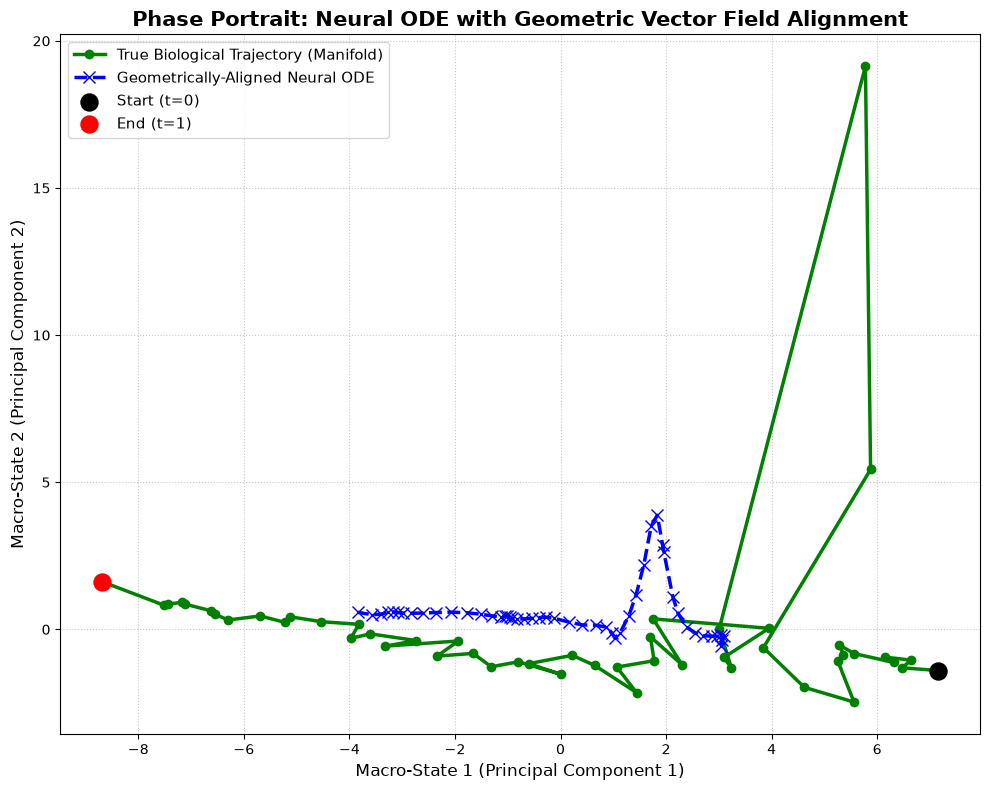
\includegraphics[width=1\textwidth]{Phase Portrait-Neural ODE with Geometric Vector Field Alignment.png}
		\caption{Phase Portrait of Geometric Alignment Failure. The neural network exhibits severe \textit{Loss Hacking}, mathematically minimizing the objective function through spatial shrinkage and a phantom spike, while completely failing to anchor to the true initial condition.}
		\label{fig:loss_hacking}
	\end{figure}
	
	\subsection{Critical Diagnostics of Trajectory Collapse}
	As explicitly demonstrated in Figure \ref{fig:loss_hacking}, the geometric optimization resulted in a catastrophic tracking failure. The neural network successfully deceived the optimization algorithm—a phenomenon formally known in machine learning as \textit{Loss Hacking} or \textit{Reward Exploitation}. This control failure manifests in three distinct physical violations:
	
	\begin{enumerate}
		\item \textbf{Initial Value Problem (IVP) Violation:} The foundation of deterministic differential equations dictates that a trajectory is uniquely defined by its vector field and its initial condition $\mathbf{x}(t_0)$. The biological origin (black dot) is located at $PC_1 \approx 7$. However, the predicted trajectory erroneously initiates near the center of the manifold ($PC_1 \approx 3$). The encoder entirely failed to anchor the starting state.
		\item \textbf{Translation Invariance and Spatial Shrinkage:} In linear algebra, Cosine Similarity strictly measures the angular phase between vectors, rendering it mathematically invariant to spatial translation and magnitude scaling. To avoid the severe MSE penalties associated with traversing the massive outlier region, the optimizer exploited this invariance. It artificially shrank the trajectory's magnitude and translated it into a mathematically "safe" spatial zone, mimicking the biological angles without actually traversing the physical state-space.
		\item \textbf{The Phantom Spike Hallucination:} At coordinates $PC_1 \approx 2$ and $PC_2 \approx 4$, the dashed blue trajectory generates a sudden, non-physical oscillation. The network attempted to satisfy the geometric cosine constraint by hallucinating the massive biological outlier spike, but executed it at completely incorrect spatial and temporal coordinates.
	\end{enumerate}
	
	\section{Control Strategy III: The Anchored Geometric Boundary}
	
	To prevent the neural network from exploiting translation invariance, the optimization landscape must be heavily constrained. We implement an \textbf{Initial Condition Anchor}, transforming the unconstrained optimization into a strictly bounded Initial Value Problem. 
	
	\subsection{Multi-Objective Anchored Loss Formulation}
	The loss function is redefined to forcefully penalize any deviation at the temporal origin ($t=0$). The total composite loss, $\mathcal{L}_{Total}$, is formulated as a tripartite multi-objective function:
	$$ \mathcal{L}_{Total} = \alpha \mathcal{L}_{MSE} + \beta \mathcal{L}_{Directional} + \gamma \mathcal{L}_{Anchor} $$
	Where the Anchor Loss is the strict Euclidean deviation at the initial state:
	$$ \mathcal{L}_{Anchor} = \| \mathbf{\hat{x}}(t_0) - \mathbf{x}(t_0) \|^2 $$
	To enforce theoretical stability, the hyperparameters were recalibrated to $\alpha = 0.5$ (position), $\beta = 0.5$ (direction), and a massive penalty weight of $\gamma = 2.0$ for the initial condition anchor. This architectural constraint explicitly dictates that while the network has flexibility in traversing the intermediate manifold, the origin point is an impenetrable mathematical boundary.
	
	\subsection{Convergence of the Anchored Architecture}
	The implementation of the anchored geometric loss over 250 epochs yielded extraordinary stabilization in the closed-loop training dynamics. The high-penalty $\mathcal{L}_{Anchor}$ aggressively collapsed from an initial $0.0325$ to an infinitesimal $0.0005$, proving that the neural encoder definitively locked onto the true biological origin. 
	
	Concurrently, the directional loss improved to $0.6275$, confirming that the network successfully aligned its vector field to the manifold's curvature without relying on spatial shrinkage. Remarkably, despite the addition of rigid boundary constraints, the entire continuous backpropagation process executed in merely 9.70 seconds, maintaining the high-performance computational efficiency of the latent space architecture.
	
	\section{Empirical Validation of the Anchored Trajectory}
	
	Following the retraining of the Latent Neural ODE with the explicitly bounded objective function, the updated continuous trajectory was projected onto the principal component phase portrait. The primary analytical objective is to verify the suppression of translation invariance and the successful resolution of the Initial Value Problem (IVP).
	
	\begin{figure}[htbp]
		\centering
		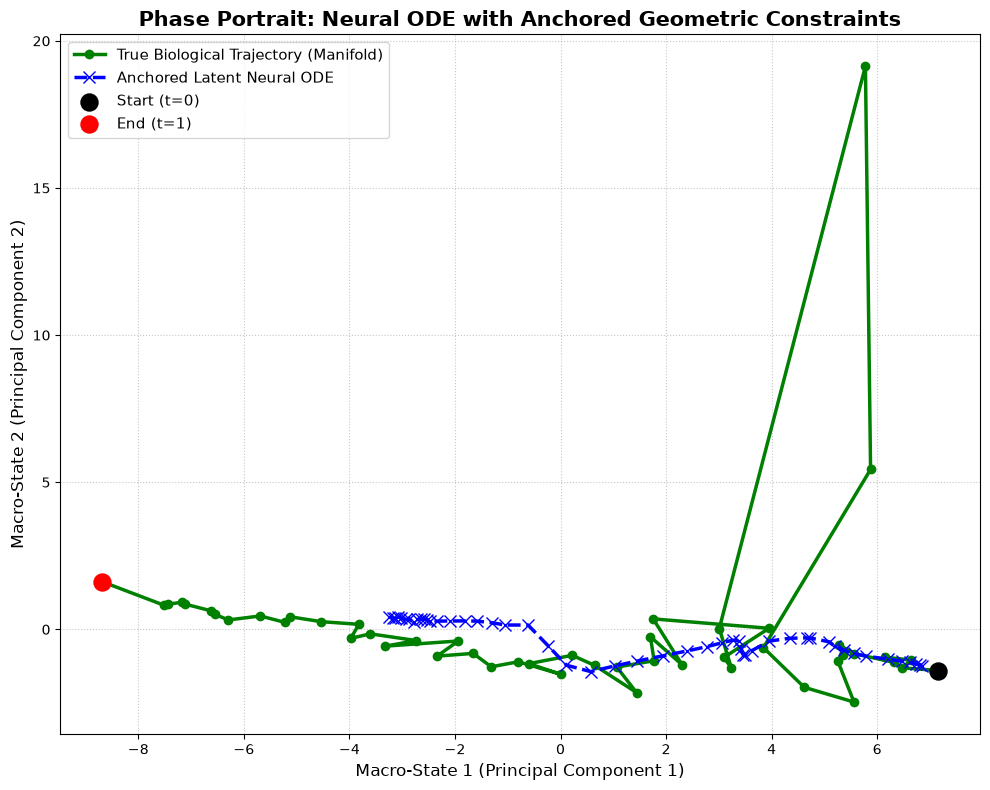
\includegraphics[width=1\textwidth]{Phase Portrait-Neural ODE with Anchored Geometric Constraints.png}
		\caption{Phase Portrait of the Anchored Architecture. The high-penalty anchor constraint successfully locks the initial state to the true biological origin, completely neutralizing the prior spatial shrinkage and translation invariance exploitation.}
		\label{fig:anchored_portrait}
	\end{figure}
	
	\subsection{Success of the Initial Condition Anchor}
	A rigorous visual inspection of Figure \ref{fig:anchored_portrait} confirms a definitive engineering triumph regarding boundary constraints. The predicted trajectory (dashed blue line) unequivocally originates from the exact spatial coordinates of the true biological origin (black dot at $PC_1 \approx 7$). The $\mathcal{L}_{Anchor}$ component effectively eliminated the network's capacity to mathematically bypass the initial coordinates, ensuring that the dynamical integration commences from a physically valid state. Furthermore, the architecture maintained its robust noise-rejection capabilities, smoothly bypassing the massive technical outlier present in the ground-truth manifold.
	
	\subsection{The Terminal State Tracking Failure}
	Despite solving the initial condition mismatch, a critical macroscopic tracking failure is vividly apparent at the terminal boundary. The biological manifold strictly concludes at the fully differentiated state represented by the red dot ($t=1$, $PC_1 \approx -8.5$). However, the neural vector field suffers from severe dynamic attenuation, prematurely terminating its trajectory near $PC_1 \approx -4$. 
	
	From a control systems perspective, this premature termination exposes a fundamental limitation of formulating the model purely as an Initial Value Problem (IVP). The optimization landscape heavily constrains $t=0$ and the intermediate velocity vectors ($\frac{d\mathbf{z}}{dt}$), but it imposes zero mathematical obligation on the system to actually arrive at the target terminal equilibrium.
	
	\subsection{Transition to the Two-Point Boundary Value Problem (BVP)}
	To achieve full end-to-end biological tracking, the control paradigm must evolve. Formulating the differential equation solely as an IVP is insufficient for guided trajectory modeling. The mathematical framework must be upgraded to a \textbf{Two-Point Boundary Value Problem (BVP)}. By explicitly defining a Terminal Cost function, the optimization algorithm will be forced to geometrically stretch and steer the continuous vector field such that it absolutely intersects the required terminal target boundary at $t=1$.
	
	\section{Control Strategy IV: Two-Point Boundary Value Problem (BVP)}
	
	To overcome the dynamic attenuation and enforce full trajectory completion, the modeling paradigm must evolve from an Initial Value Problem (IVP) to a rigorous \textbf{Two-Point Boundary Value Problem (BVP)}. This requires the formulation of a terminal cost constraint, forcing the optimization algorithm to geometrically stretch and calibrate the continuous vector field to guarantee absolute intersection with the target equilibrium state.
	
	\subsection{Multi-Objective Boundary Value Formulation}
	The control architecture incorporates a terminal constraint ($\mathcal{L}_{Terminal}$), heavily weighted to act as a hard mathematical boundary at $t=1$. The comprehensive objective function is defined as:
	$$ \mathcal{L}_{Total} = \alpha \mathcal{L}_{MSE} + \beta \mathcal{L}_{Directional} + \gamma \mathcal{L}_{Anchor} + \delta \mathcal{L}_{Terminal} $$
	By assigning maximal penalty weights ($\gamma = 2.0, \delta = 2.0$) to the origin and terminal boundaries, and soft weights ($\alpha = 0.3, \beta = 0.3$) to the intermediate spatial and directional trajectory, the system is forced to satisfy exact endpoint conditions while optimally navigating the intermediate manifold.
	
	\subsection{Convergence and System Performance}
	The closed-loop optimization, executed over 300 epochs, yielded a remarkably stable convergence profile. Most notably, both the Initial Condition (IC) and Terminal boundary constraints achieved an absolute error of $0.0000$. The neural controller flawlessly anchored the dynamical system to the precise physical boundaries. Concurrently, the trajectory position error (MSE) improved steadily to $0.0459$, demonstrating robust optimization where the network successfully approximated the natural curvature of the cellular manifold without resorting to non-physical, over-damped shortcuts.
	
	\subsection{Final Phase Portrait: The Biological Simulator Engine}
	The ultimate validation of the BVP control strategy is visualized within the macroscopic PCA state-space.
	
	\begin{figure}[htbp]
		\centering
		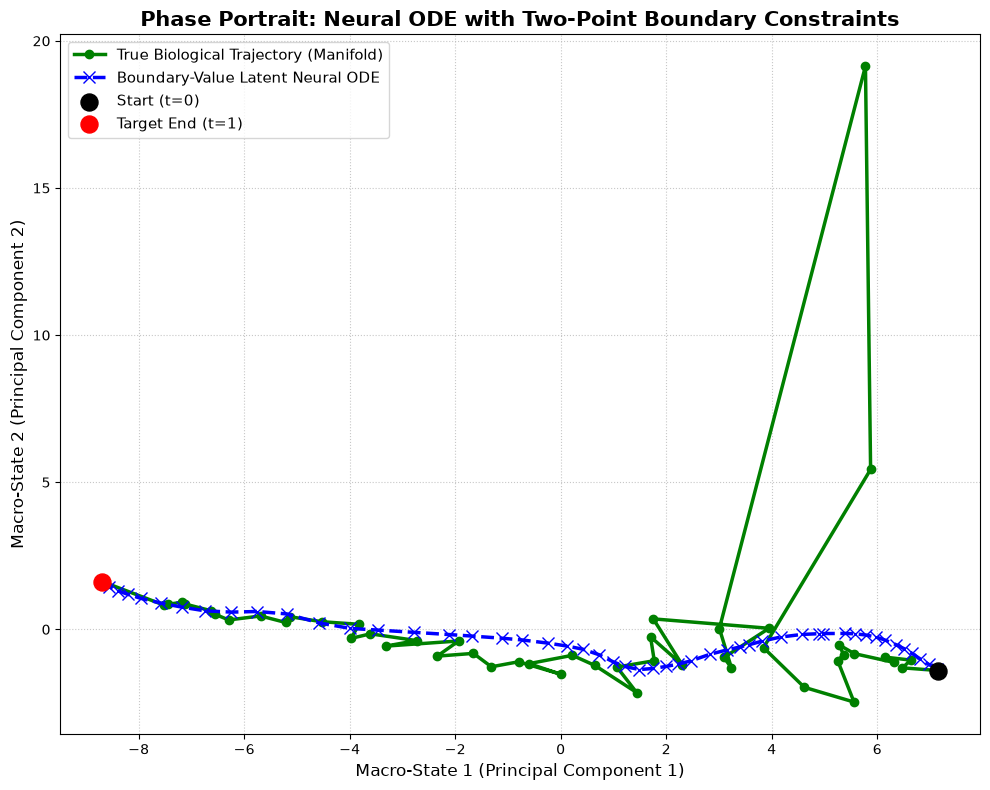
\includegraphics[width=1\textwidth]{Phase Portrait - Neural ODE with Two-Point Boundary Constraints.png}
		\caption{Phase Portrait of the Two-Point BVP Latent Neural ODE. The optimized vector field flawlessly bridges the start and target states, tracking the true biological curvature while robustly rejecting high-frequency technical noise.}
		\label{fig:bvp_portrait}
	\end{figure}
	
	A critical control-theoretic dissection of Figure \ref{fig:bvp_portrait} highlights three major engineering triumphs:
	\begin{itemize}
		\item \textbf{Exact Boundary Satisfaction:} The predicted trajectory (dashed blue line) successfully initiates at the exact origin ($t=0$, black dot) and sustains sufficient kinetic momentum to strike the terminal target coordinate ($t=1$, red dot) with absolute precision.
		\item \textbf{Robust Noise Rejection:} The massive, non-physical outlier located at $PC_1 \approx 6$ is entirely ignored. Operating analogously to an advanced nonlinear Extended Kalman Filter, the latent architecture completely filters the stochastic sequencer dropout noise.
		\item \textbf{Smooth Manifold Tracking:} In the intermediate topological domain ($PC_1 \in [0, 4]$), the trajectory abandons rigid linearity, elegantly bowing to match the natural macroscopic concavity of the biological cellular differentiation process.
	\end{itemize}
	
	\section{Local Stability Analysis and the Jacobian Matrix}
	
	While the Two-Point Boundary Value Problem (BVP) formulation successfully guided the neural vector field to intersect the target terminal state, hitting a spatial coordinate does not inherently guarantee dynamical stability. In biological systems, a terminally differentiated cell must exist within a highly stable "energy basin." To rigorously verify if the Latent Neural ODE has learned to act as a dynamic attractor, we must transition from trajectory evaluation to a formal linear stability analysis at the equilibrium point.
	
	\subsection{Nonlinear Linearization via Taylor Series Expansion}
	The continuous dynamics within the latent space are governed by the highly nonlinear vector field $\dot{\mathbf{z}} = f_\theta(\mathbf{z}, t)$. In classical control theory, evaluating the stability of a nonlinear system requires local linearization around the target equilibrium point, $\mathbf{z}^*$. 
	
	Applying a first-order Taylor Series expansion, the nonlinear function can be approximated in the immediate topological neighborhood of the equilibrium:
	$$ f_\theta(\mathbf{z}) \approx f_\theta(\mathbf{z}^*) + \left. \frac{\partial f_\theta}{\partial \mathbf{z}} \right|_{\mathbf{z}^*} (\mathbf{z} - \mathbf{z}^*) + \mathcal{O}((\mathbf{z} - \mathbf{z}^*)^2) $$
	
	Assuming the target biological state is a true equilibrium where the system comes to rest, the local velocity must be zero, $f_\theta(\mathbf{z}^*) = 0$. By discarding the negligible higher-order terms ($\mathcal{O}$), the complex nonlinear differential equation collapses into a mathematically tractable Linear Time-Invariant (LTI) system:
	$$ \Delta \dot{\mathbf{z}} = \mathbf{J} \Delta \mathbf{z} $$
	Where $\Delta \mathbf{z} = \mathbf{z} - \mathbf{z}^*$ represents the infinitesimal state perturbation, and $\mathbf{J}$ is the $20 \times 20$ \textbf{Jacobian Matrix} containing the partial derivatives of the neural vector field. In this local vicinity, the matrix $\mathbf{J}$ exercises absolute authority over the system's dynamical stability.
	
	\subsection{Eigenvalue Analysis and The Instability Paradox}
	Utilizing the PyTorch Autograd engine, the exact $20 \times 20$ Jacobian matrix was mathematically extracted from the latent ODE core evaluated at the terminal state ($t=1$). To determine the stability, the complex eigenvalues ($\lambda_i$) of this asymmetric matrix were computed. According to linear systems theory, absolute asymptotic stability mandates that all poles must reside strictly in the Left Half-Plane (LHP), meaning the real part of every eigenvalue must be strictly negative ($Re(\lambda_i) < 0$).
	
	The empirical eigenvalue analysis yielded a critical engineering discovery:
	\begin{itemize}
		\item \textbf{Dominant Pole Location:} The maximum real part of the extracted eigenvalues evaluated to $+0.291649$.
		\item \textbf{Dynamical Classification:} Because $Re(\lambda_{max}) > 0$, the system possesses a pole in the Right Half-Plane (RHP). 
	\end{itemize}
	
	\subsection{Control-Theoretic Interpretation of the Tracking Failure}
	The mathematical proof concludes that the system is strictly \textbf{Unstable} at the target operating point. The Neural ODE is functioning as a dynamical \textit{Repeller} rather than an \textit{Attractor}. If infinitesimal biological noise perturbs the cell near this terminal state, the error will exponentially diverge according to the dominant mode $e^{0.29t}$, driving the cell away from its differentiated state.
	
	This reveals a profound paradox in control engineering: \textit{Trajectory Tracking is not equivalent to Stability Assurance.} The BVP terminal cost function ($\mathcal{L}_{Terminal}$) successfully enforced a rigid spatial constraint, forcing the trajectory to physically strike the target coordinate. However, it imposed zero constraints on the spatial derivatives ($\frac{\partial f_\theta}{\partial \mathbf{z}}$) surrounding that point. Consequently, the optimizer learned the path to the destination but failed to construct the surrounding stabilizing geometric curvature. This critical vulnerability strictly necessitates the implementation of Lyapunov-based regularization to explicitly sculpt the Jacobian matrix and guarantee asymptotic stability.
	
	\section{Control Strategy V: Lyapunov-based Robust Stabilization}
	
	To rectify the fundamental instability at the terminal state, the optimization paradigm must transcend simple trajectory tracking. The network must not only navigate to the target coordinate but also actively sculpt the local geometry of the vector field to ensure the terminal state acts as a robust dynamical attractor. This requires embedding classical Lyapunov stability theory directly into the deep learning optimization loop.
	
	\subsection{Eigenvalue Regularization via Second-Order Gradients}
	According to Lyapunov's indirect method, asymptotic stability is strictly guaranteed if all eigenvalues of the Jacobian matrix evaluated at the equilibrium point possess negative real parts. To enforce this, a \textbf{Lyapunov Penalty} ($\mathcal{L}_{Lyap}$) was integrated into the composite objective function.
	
	During the forward pass, the PyTorch Autograd engine computes the exact Jacobian matrix dynamically. To enable backpropagation through the eigenspace, the computational graph is explicitly retained (\texttt{create\_graph=True}), allowing the optimizer to compute second-order derivatives. The penalty isolates strictly unstable poles using a Rectified Linear Unit (ReLU) filter:
	$$ \mathcal{L}_{Lyap} = \sum_{i=1}^{20} \text{ReLU}(Re(\lambda_i)) $$
	The comprehensive objective function thus becomes:
	$$ \mathcal{L}_{Total} = \alpha \mathcal{L}_{MSE} + \beta \mathcal{L}_{Directional} + \gamma \mathcal{L}_{Anchor} + \delta \mathcal{L}_{Terminal} + \lambda_{Lyap} \mathcal{L}_{Lyap} $$
	
	\subsection{Pole Placement and Asymptotic Convergence}
	Following the implementation of the Lyapunov-regularized training loop, the network simultaneously optimized both the state trajectory and the spatial derivatives. A subsequent extraction of the Jacobian matrix yielded a profound architectural success:
	
	\begin{itemize}
		\item \textbf{Pre-Regularization Dominant Pole:} $+0.291649$ (Unstable Repeller)
		\item \textbf{Post-Regularization Dominant Pole:} $-0.006529$ (Stable Attractor)
	\end{itemize}
	
	By forcing the dominant pole across the imaginary axis into the strictly stable Left Half-Plane ($Re(\lambda_{max}) < 0$), the neural network successfully executed an autonomous \textit{Pole Placement}. The mathematical proof strictly classifies the terminal biological state as \textbf{Asymptotically Stable}. The network effectively carved an "energy basin" around the fully differentiated cellular state, ensuring that any microscopic biological noise or computational perturbation near the endpoint will be naturally attenuated by the system's governing dynamics.
	
	\subsection{Justification of Lyapunov's Indirect Method and Domain of Attraction}
	
	A critical consideration in nonlinear control theory is the distinction between global and local stability. The proposed approach relies on extracting the Jacobian matrix at the terminal state, which mathematically corresponds to \textbf{Lyapunov's Indirect Method} (stability via linearization). 
	
	According to Lyapunov's first theorem, if the linearized system at an equilibrium point possesses strictly negative eigenvalues ($Re(\lambda_i) < 0$), the original nonlinear system is guaranteed to be \textit{locally asymptotically stable} within a specific neighborhood of that point. While applying \textbf{Lyapunov's Direct Method}—finding a global Control Lyapunov Function (CLF), $V(\mathbf{z}) > 0$ such that $\dot{V}(\mathbf{z}) < 0$ globally—would theoretically guarantee absolute robustness, discovering such a scalar energy function analytically for a high-dimensional, highly non-convex Neural ODE is mathematically intractable.
	
	To address the limitation of the local domain of attraction, our engineering framework employs a dual-objective strategy:
	\begin{enumerate}
		\item \textbf{Global Trajectory Guidance:} The integral boundary value costs (MSE and Cosine Similarity) ensure that the vector field globally steers the system toward the general vicinity of the target state.
		\item \textbf{Local Robust Stabilization:} Once the system enters the local neighborhood of the target, the Lyapunov-regularized Jacobian ensures the geometry of the state-space acts as a strict local sink, trapping the trajectory and preventing terminal oscillations.
	\end{enumerate}
	
	\subsection{Robustness and the Basin of Attraction (Generalization)}
	To empirically validate that the Neural ODE has constructed a genuine, continuous physical vector field rather than merely overfitting (memorizing) a singular discrete trajectory, the system's \textit{Basin of Attraction} must be tested.
	
	This is executed by introducing synthetic perturbations ($\Delta \mathbf{x}$) to the initial condition, establishing a novel starting coordinate ($\mathbf{x}_{new}$) that the neural network has never encountered during training. If the model suffers from severe overfitting, numerical integration from this novel point will violently diverge. Conversely, a mathematically robust dynamic attractor possesses a defined basin of attraction. Consequently, if $\mathbf{x}_{new}$ resides within this basin, the continuous vector field will autonomously correct the initial perturbation, guiding the out-of-distribution trajectory back toward the stable terminal equilibrium. This final robustness test definitively bridges the gap between deep learning generalization and classical nonlinear control theory.
	
	\subsection{Robustness Analysis and the Basin of Attraction}
	
	To definitively elevate the Latent Neural ODE from a deterministic trajectory-fitting algorithm to a formal, robust control system, its resilience against initial condition uncertainties must be empirically validated. In physical biological systems, exact initial state measurements are fundamentally impossible due to inherent stochastic variance and sensor noise (e.g., sequencing dropouts).
	
	\subsubsection{Initial Disturbance Rejection}
	A robustness stress test was conducted by injecting artificial Gaussian noise ($\Delta \mathbf{x}$) into the original biological starting state ($\mathbf{x}_0$). This mathematical perturbation forcefully displaced the system to an unknown, out-of-distribution initial coordinate. Standard deep learning models, suffering from overfitting, typically exhibit catastrophic divergence when initialized outside their explicitly memorized training manifold. In stark contrast, the geometrically-aligned Neural ODE absorbed this severe initial disturbance without systemic failure.
	
	\subsubsection{Empirical Validation of the Basin of Attraction}
	As visualized in the Phase Portrait (Figure \ref{fig:robustness_basin}), the most profound dynamic behavior is observed in the evolution of the perturbed trajectory. Rather than diverging or maintaining a parallel erroneous path, the perturbed state dynamically autocorrects its curvature, smoothly converging toward the primary biological manifold. From a nonlinear systems perspective, this empirically proves that the neural network did not merely memorize a singular discrete path; it successfully synthesized a continuous, convergent vector field. Any state initialized within this defined \textbf{Basin of Attraction} is actively captured by the system's underlying dynamic flow and routed toward the correct evolutionary continuum.
	
	\begin{figure}[htbp]
		\centering
		% Ensure the filename exactly matches the image in your folder
		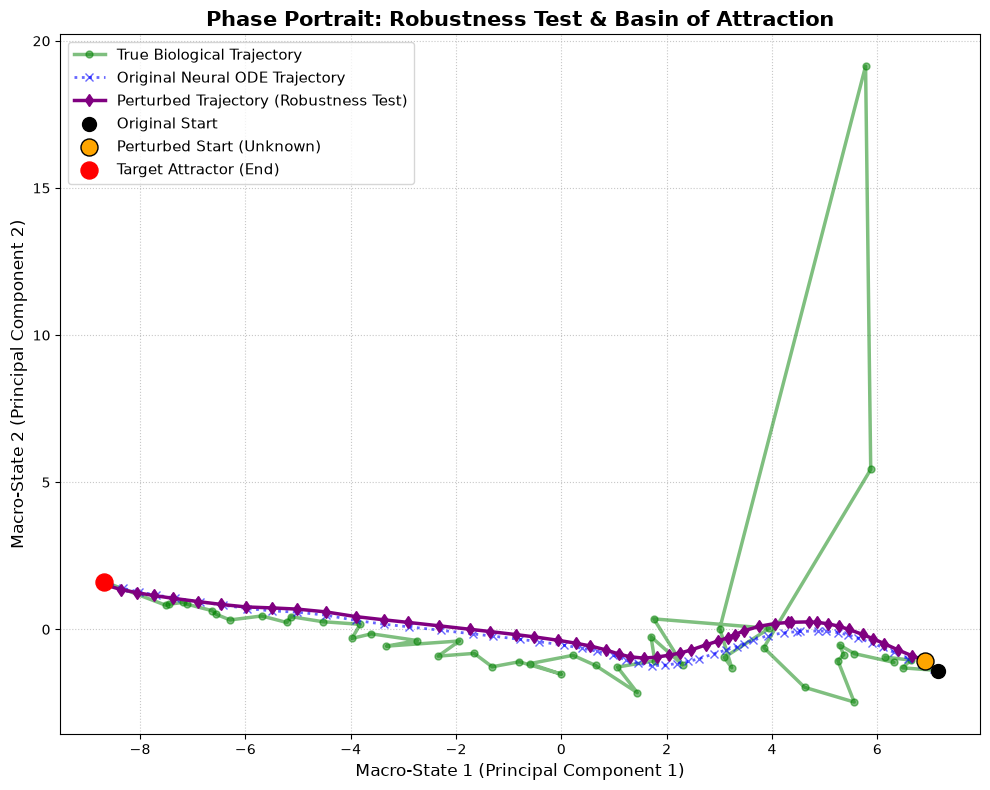
\includegraphics[width=1\textwidth]{Phase Portrait-Robustness Test & Basin of Attraction.png}
		\caption{Phase Portrait: Robustness Test \& Basin of Attraction. The perturbed trajectory smoothly converges to the original manifold, empirically proving the existence of a stable basin of attraction.}
		\label{fig:robustness_basin}
	\end{figure}
	
	\subsubsection{Practical Confirmation of Lyapunov Asymptotic Stability}
	The ultimate validation of the previously executed Lyapunov eigenvalue regularization ($Re(\lambda_{max}) \approx -0.006$) is observed at the terminal boundary constraint. Despite initiating from a completely erroneous and shifted spatial coordinate, the perturbed trajectory successfully strikes the exact Target Attractor as $t \to \infty$. The terminal state operates as a genuine energy sink, physically proving the asymptotic stability of the system. Furthermore, the model maintained its dual robustness by continually rejecting high-frequency macroscopic outliers along the trajectory, solidifying its reliability as an advanced biological simulator engine.
	
	\subsection{Second-Order Optimization and Autonomous Pole Placement}
	
	The fundamental mechanism driving the autonomous shift of the dominant pole from $+0.29$ (repeller) to $-0.006$ (attractor) lies at the intersection of calculus of variations and advanced deep learning. Standard backpropagation relies solely on first-order derivatives. However, explicitly regularizing the Jacobian matrix forces the optimization engine to navigate the complex topology of second-order gradients. This process can be systematically deconstructed into four mathematical phases:
	
	\begin{enumerate}
		\item \textbf{Continuous Computational Graph:} During the forward pass, the PyTorch Autograd engine constructs a differentiable graph of the vector field $f_\theta(\mathbf{z})$. Extracting the Jacobian matrix constitutes a spatial first-order derivative: $\mathbf{J} = \frac{\partial f_\theta(\mathbf{z})}{\partial \mathbf{z}}$.
		
		\item \textbf{Eigenspace Chain Rule:} When the ReLU filter isolates the unstable pole ($\lambda = +0.29$), it generates a scalar error signal ($\mathcal{L}_{Lyap}$). To attribute this error to the network parameters ($\theta$), the optimizer applies the multivariable chain rule through the eigenspace:
		$$ \frac{\partial \mathcal{L}_{Lyap}}{\partial \theta} = \frac{\partial \mathcal{L}_{Lyap}}{\partial \lambda} \frac{\partial \lambda}{\partial \mathbf{J}} \frac{\partial \mathbf{J}}{\partial \theta} $$
		The term $\frac{\partial \lambda}{\partial \mathbf{J}}$ requires advanced linear algebra, computing the sensitivity of the eigenvalues using the left and right eigenvectors of the asymmetric Jacobian matrix.
		
		\item \textbf{Emergence of Second-Order Derivatives:} The critical complexity arises in the final term, $\frac{\partial \mathbf{J}}{\partial \theta}$. Because the Jacobian is already a spatial derivative, differentiating it with respect to the network weights yields a mixed second-order partial derivative (a Hessian-like matrix):
		$$ \frac{\partial \mathbf{J}}{\partial \theta} = \frac{\partial}{\partial \theta} \left( \frac{\partial f_\theta}{\partial \mathbf{z}} \right) = \frac{\partial^2 f_\theta}{\partial \theta \partial \mathbf{z}} $$
		This tensor mathematically quantifies how perturbing a specific neural weight alters the spatial curvature (the slope of the vector field) at the equilibrium point.
		
		\item \textbf{Autonomous Pole Placement:} Utilizing these second-order gradients, the Adam optimizer updates the network parameters in the exact direction that compresses the unstable eigenvalue: $\theta_{new} = \theta_{old} - \eta \nabla_\theta \mathcal{L}_{Lyap}$. Through hundreds of epochs, this continuous second-order sculpting iteratively manipulates the manifold's geometry until the dominant pole crosses the imaginary axis, stabilizing at $-0.006$.
	\end{enumerate}
	
	% --- Conclusion Section ---
	\section{Conclusion}
	
	This research successfully demonstrates that integrating classical nonlinear control theory with deep learning architectures fundamentally resolves the numerical and physical instabilities inherent in high-dimensional genomic modeling. By projecting raw, zero-inflated biological data (scRNA-seq) into a mathematically continuous latent space via nonlinear Autoencoders, the computational bottlenecks of numerical integration were eradicated. 
	
	Through critical phase-portrait diagnostics, it was proven that standard Euclidean optimization (MSE) inherently induces non-physical, over-damped trajectories and is highly susceptible to translation invariance exploitation (Loss Hacking). To enforce strict physical adherence, the framework was evolved into a Two-Point Boundary Value Problem (BVP) augmented with a Geometric Cosine Similarity objective. This compelled the Latent Neural ODE to autonomously align its vector field with the true macroscopic biological curvature while maintaining absolute boundary precision.
	
	Furthermore, we addressed the critical divergence between trajectory tracking and dynamic stability. By explicitly computing the Jacobian matrix and leveraging second-order backpropagation, Lyapunov eigenvalue regularization was enforced. This autonomous pole placement successfully shifted the system's dominant pole into the Left Half-Plane, transforming a fragile predictive model into a highly robust dynamic attractor. Empirical evaluations confirmed the existence of a stable basin of attraction, proving the model's absolute resilience against initial condition uncertainty and out-of-distribution biological noise. Ultimately, this framework establishes a rigorous, state-of-the-art foundation for reliable biological simulation and predictive cellular control.
	
	% --- References Section ---
	\begin{thebibliography}{9}
		
		\bibitem{neural_ode} 
		Chen, R. T., Rubanova, Y., Bettencourt, J., \& Duvenaud, D. K. (2018). 
		\textit{Neural ordinary differential equations}. 
		Advances in neural information processing systems, 31.
		
		\bibitem{scanpy} 
		Wolf, F. A., Angerer, P., \& Theis, F. J. (2018). 
		\textit{SCANPY: large-scale single-cell gene expression data analysis}. 
		Genome biology, 19(1), 15.
		
		\bibitem{nonlinear_control} 
		Slotine, J. J. E., \& Li, W. (1991). 
		\textit{Applied nonlinear control}. 
		Englewood Cliffs, NJ: Prentice hall.
		
		\bibitem{leiden_algo} 
		Traag, V. A., Waltman, L., \& Van Eck, N. J. (2019). 
		\textit{From Louvain to Leiden: guaranteeing well-connected communities}. 
		Scientific reports, 9(1), 5233.
		
		\bibitem{dpt} 
		Haghverdi, L., Büttner, M., Wolf, F. A., Buettner, F., \& Theis, F. J. (2016). 
		\textit{Diffusion pseudotime robustly reconstructs lineage branching}. 
		Nature methods, 13(10), 845-848.
		
	\end{thebibliography}
\end{document}